\section{Introduction}

A detailed explanation for the estimation of the Z$\rightarrow\nu\bar{\nu}$+jets background is presented in this chapter. The following estimation procedure builds upon the 2016 SUSY analysis summarized in \autoref{AnalysisChap} and aims to refine the overall background calculation as well as reduce the uncertainties associated with the previous method. To accomplish this, an additional $\gamma$+jets CS is used in conjunction with the tight Z$\rightarrow\mu^{+}\mu^{-}$ control region used in the 2016 analysis estimation. The new $\gamma$+jets CS provides a more data-driven estimation procedure with the added benefit of a substantially larger production cross-section than Z+jets processes\cite{Zgamma}.  

\section{The Irreducible Z$\rightarrow\nu\bar{\nu}$ Background}

An important source of background in searches for SUSY in the 0-lepton final state comes from events in which a Z boson, accompanied by jets, decays into a pair of neutrinos (Z$\rightarrow\nu\bar{\nu}$+jets). The resulting final state is comprised of a large $p_\text{T}^{miss}$ (from the neutrino pair) and multiple hadron jets, closely mimicking the SUSY signal. For similar searches, the Z$\rightarrow\nu\bar{\nu}$ contribution can make up a large portion of the background in many of the search bin regions (higher than 50\% in some regions)\cite{OtherAna1,OtherAna2}, and can compose up to about a third of the total SM background. For this particular analysis, the Z$\rightarrow\nu\bar{\nu}$ accounts for about 17\% of the total SM background and owes its low value to the dedicated top-tagging algorithm outlined in \autoref{TopTaggerSec}.\\

There are several different methods that have been developed to estimate the Z$\rightarrow\nu\bar{\nu}$+jets background\cite{ZInv}. Two of the commonly used methods involve the use of a control region dominated by Z$\rightarrow ll$+jets, where the $l$ stands for lepton (either a muon or an electron, in this case) or $\gamma$+jets events. The Z$\rightarrow ll$ channel has the advantage of having very similar kinematics to the Z$\rightarrow\nu\bar{\nu}$ region but suffers from low statistics (due in part to its small branching ratio), specially in the tight search regions used in typical SUSY searches. On the other hand, the $\gamma$+jets region has a much higher production cross-section but involves a completely different process. The hybrid method described in this chapter makes use of both control regions in order to estimate the Z$\rightarrow\nu\bar{\nu}$ background corrections, and aims to improve on the results of the 2016 method described in \autoref{ZnunuSection}.

\begin{figure}[H]
\begin{center}
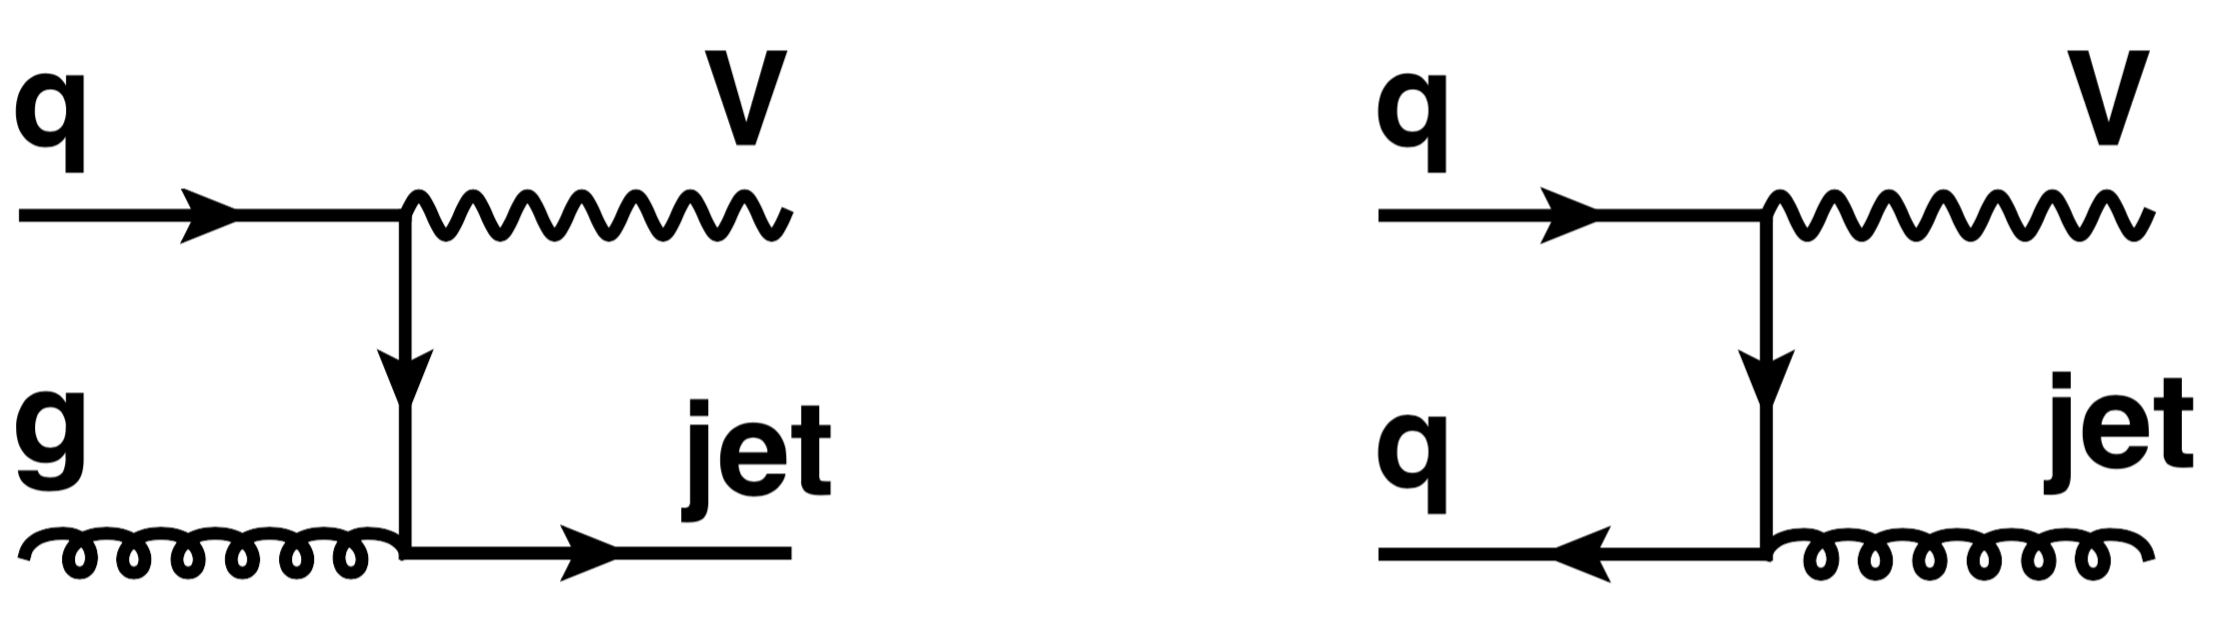
\includegraphics[width=0.8\textwidth]{Ztogamma.png}
\end{center}
\vspace{-1em}
\caption[Leading-order Feynman diagrams for Z+ jets and $\gamma$+ jets processes.]{Leading-order Feynman diagrams for Z+ jets and $\gamma$+ jets processes. The `V' in the figure can represent either Z or $\gamma$.}
\label{Ztogamma}
\end{figure}

\section{The Loose $\gamma$+jets Control Region}

The loose $\gamma+$jets control region, as well as the photon ID/isolation selection, is described in this section. The $\gamma+$jets control region is chosen with the purpose of substituting the loose muon control region used in the 2016 version of this analysis for the calculation of the shape correction scale factors applied to the final estimation of the Z$\rightarrow\nu\bar{\nu}$ background. The $\gamma+$jets control region is presumed to be better suited for this estimation due to having a much higher cross-section and therefore, an expected reduction in the statistical and systematic uncertainties associated to the shape correction factors are expected. 

\subsection{Photon ID and Isolation}\label{photonID}

Three different working points are provided by the CMS EGM physics object group (POG) for simple cut-based photon identification\cite{photonID}. The three working points, called loose, medium and tight, are chosen according to the requirements of the particular analysis and differ on the amount of background rejection they offer, as well as on their average photon selection efficiency. The higher the efficiency of a given ID, the lower the amount of background that is rejected, and vice-versa. \autoref{IDtable} shows the cut values that are applied to photons that are found within both the ECAL barrel and endcap range. The associated values to the efficiency and the background rejection rate are shown for each of the three different photon ID selections.\\

In order to obtain the high efficiency and background rejection rates shown, a robust set of identification and isolation criteria are selected. A total of five parameters are used for this simple cut based method. For photon identification, the H/E and the $\sigma I\eta I\eta$ variables are found to provide the best results. The H/E parameter is defined as the ratio of the HCAL tower energy over the ECAL seed cluster energy. A threshold value is selected on H/E to remove background from electrons that are detected in both the ECAL and HCAL but have no reconstructed track\cite{egamma}. The $\sigma I\eta I\eta$ variable is known as the photon shower shape variable and is defined in the ECAL as the energy weighted standard deviation of a single crystal within the 5 $\times$ 5 crystal $\eta$ range, centered around the crystal with maximum energy\cite{showershape}. This variable is a key component in the identification of both electrons and photons since it provides a measure of the shower width where most of the energy has been deposited in a given ECAL crystal.

\begin{table}[H]
\centering
\caption{Identification and isolation cut values for photons provided by the CMS EGM POG. Values are provided for the three working points described (loose, medium and tight) for both the ECAL barrel and endcaps. The photon selection efficiency of the three working points, as well as their associated background rejection rate, are provided.}
\label{IDtable}
\resizebox{\textwidth}{!}{%
\begin{tabular}{|l|l|l|l|}
\hline
\textbf{Barrel} & \textbf{Loose (90.06\%)} & \textbf{Medium (80.19\%)} & \textbf{Tight (70.01\%)} \\ \hline
\textbf{Background Rejection} & \textbf{Loose (85.73\%)} & \textbf{Medium (88.87\%)} & \textbf{Tight (90.66\%)} \\ \hline
H/E & 0.105 & 0.035 & 0.020 \\ \hline
$\sigma I\eta I\eta$ & 0.0103 & 0.0103 & 0.0103 \\ \hline
\begin{tabular}[c]{@{}l@{}}$\rho$-corrected PF charged \\ hadron isolation\end{tabular} & 2.839 & 1.416 & 1.158 \\ \hline
\begin{tabular}[c]{@{}l@{}}$\rho$-corrected PF neutral \\ hadron isolation\end{tabular} & \begin{tabular}[c]{@{}l@{}}$9.188 + 0.0126 \cdot{p_\text{T}^\gamma} +$ \\ $0.000026\cdot{p_\text{T}^\gamma}^2$\end{tabular} & \begin{tabular}[c]{@{}l@{}}$2.491 + 0.0126 \cdot{p_\text{T}^\gamma} +$ \\ $0.000026\cdot{p_\text{T}^\gamma}^2$\end{tabular} & \begin{tabular}[c]{@{}l@{}}$1.267 + 0.0126 \cdot{p_\text{T}^\gamma} +$ \\ $0.000026\cdot{p_\text{T}^\gamma}^2$\end{tabular} \\ \hline
\begin{tabular}[c]{@{}l@{}}$\rho$-corrected PF photon \\ isolation\end{tabular} & $2.956 + 0.0035 \cdot{p_\text{T}^\gamma}$ & $2.952 + 0.0040 \cdot{p_\text{T}^\gamma}$ & $2.065 + 0.0035 \cdot{p_\text{T}^\gamma}$ \\ \hline
\end{tabular}%
}

\vspace{1em}

\centering
\resizebox{\textwidth}{!}{%
\begin{tabular}{|l|l|l|l|}
\hline
\textbf{End Cap} & \textbf{Loose (90.81\%)} & \textbf{Medium (80.06\%)} & \textbf{Tight (70.11\%)} \\ \hline
\textbf{Background Rejection} & \textbf{Loose (76.90\%)} & \textbf{Medium (81.50\%)} & \textbf{Tight (84.34\%)} \\ \hline
H/E & 0.029 & 0.027 & 0.025 \\ \hline
$\sigma I\eta I\eta$ & 0.0276 & 0.0271 & 0.0271 \\ \hline
\begin{tabular}[c]{@{}l@{}}$\rho$-corrected PF charged \\ hadron isolation\end{tabular} & 2.150 & 1.012 & 0.575 \\ \hline
\begin{tabular}[c]{@{}l@{}}$\rho$-corrected PF neutral \\ hadron isolation\end{tabular} & \begin{tabular}[c]{@{}l@{}}$10.471 + 0.0119 \cdot{p_\text{T}^\gamma} +$ \\ $0.000025\cdot{p_\text{T}^\gamma}^2$\end{tabular} & \begin{tabular}[c]{@{}l@{}}$9.131 + 0.0119 \cdot{p_\text{T}^\gamma} +$ \\ $0.000025\cdot{p_\text{T}^\gamma}^2$\end{tabular} & \begin{tabular}[c]{@{}l@{}}$8.916 + 0.0119 \cdot{p_\text{T}^\gamma} +$ \\ $0.000025\cdot{p_\text{T}^\gamma}^2$\end{tabular} \\ \hline
\begin{tabular}[c]{@{}l@{}}$\rho$-corrected PF photon \\ isolation\end{tabular} & $4.895 + 0.0040\cdot{p_\text{T}^\gamma}$ & $4.095 + 0.0040 \cdot{p_\text{T}^\gamma}$ & $3.272 + 0.0040 \cdot{p_\text{T}^\gamma}$ \\ \hline
\end{tabular}
}
\end{table}

The other three parameters considered, comprise the isolation portion of the photon selection cuts. These are the $\rho$-corrected particle flow (PF) charged hadron, neutral hadron and photon isolation parameters. As can be seen from \autoref{IDtable}, two of these parameters (the neutral hadron and photon isolation) have a dependence on $p_\text{T}^\gamma$. These cuts are used to ensure that the identified photon is well isolated within its own cone and by rejecting photons that are identified within close proximity to either a charged or a neutral hadron\cite{PFref2}. The value $\rho$ included in the name of each of these parameters refers to the total pileup density\cite{RhoRef}. Therefore, the term ``$\rho$-corrected'' implies that these values, which are sensitive to the residual contamination that arises from pile-up, have been corrected to include these contributions.

\subsection{Photon Selection}\label{photonSelection}
The event selection process for the $\gamma$+jets control region starts with photon candidates that have a $p_\text{T} > 200$ GeV and are within the acceptance range of the CMS ECAL (given by $|\eta| < 1.4442$ for the barrel and $1.566 < |\eta| < 2.5$ for the endcaps). The photons are subjected to pass the loose ID/isolation cuts described in \autoref{photonID} in order to remove $\sim85\%$ of the background processes and obtain a prompt photon sample that is $\sim90\%$ pure, on average. Additional restrictions include some of the same requirements imposed on the signal baseline selection discussed in \autoref{baseline}. These include $N_j \geq 4$, an $H_\text{T} > 300$ GeV, the $\Delta\phi$ requirements for leading jets and the lepton vetoes described in \autoref{lepVeto}. The lepton veto, in particular, greatly improves the prompt photon selection by removing many of the events in the simulated samples where a lepton gets misidentified as a photon.

\begin{figure}[H]
\begin{center}
\begin{minipage}[b]{0.45\textwidth}
    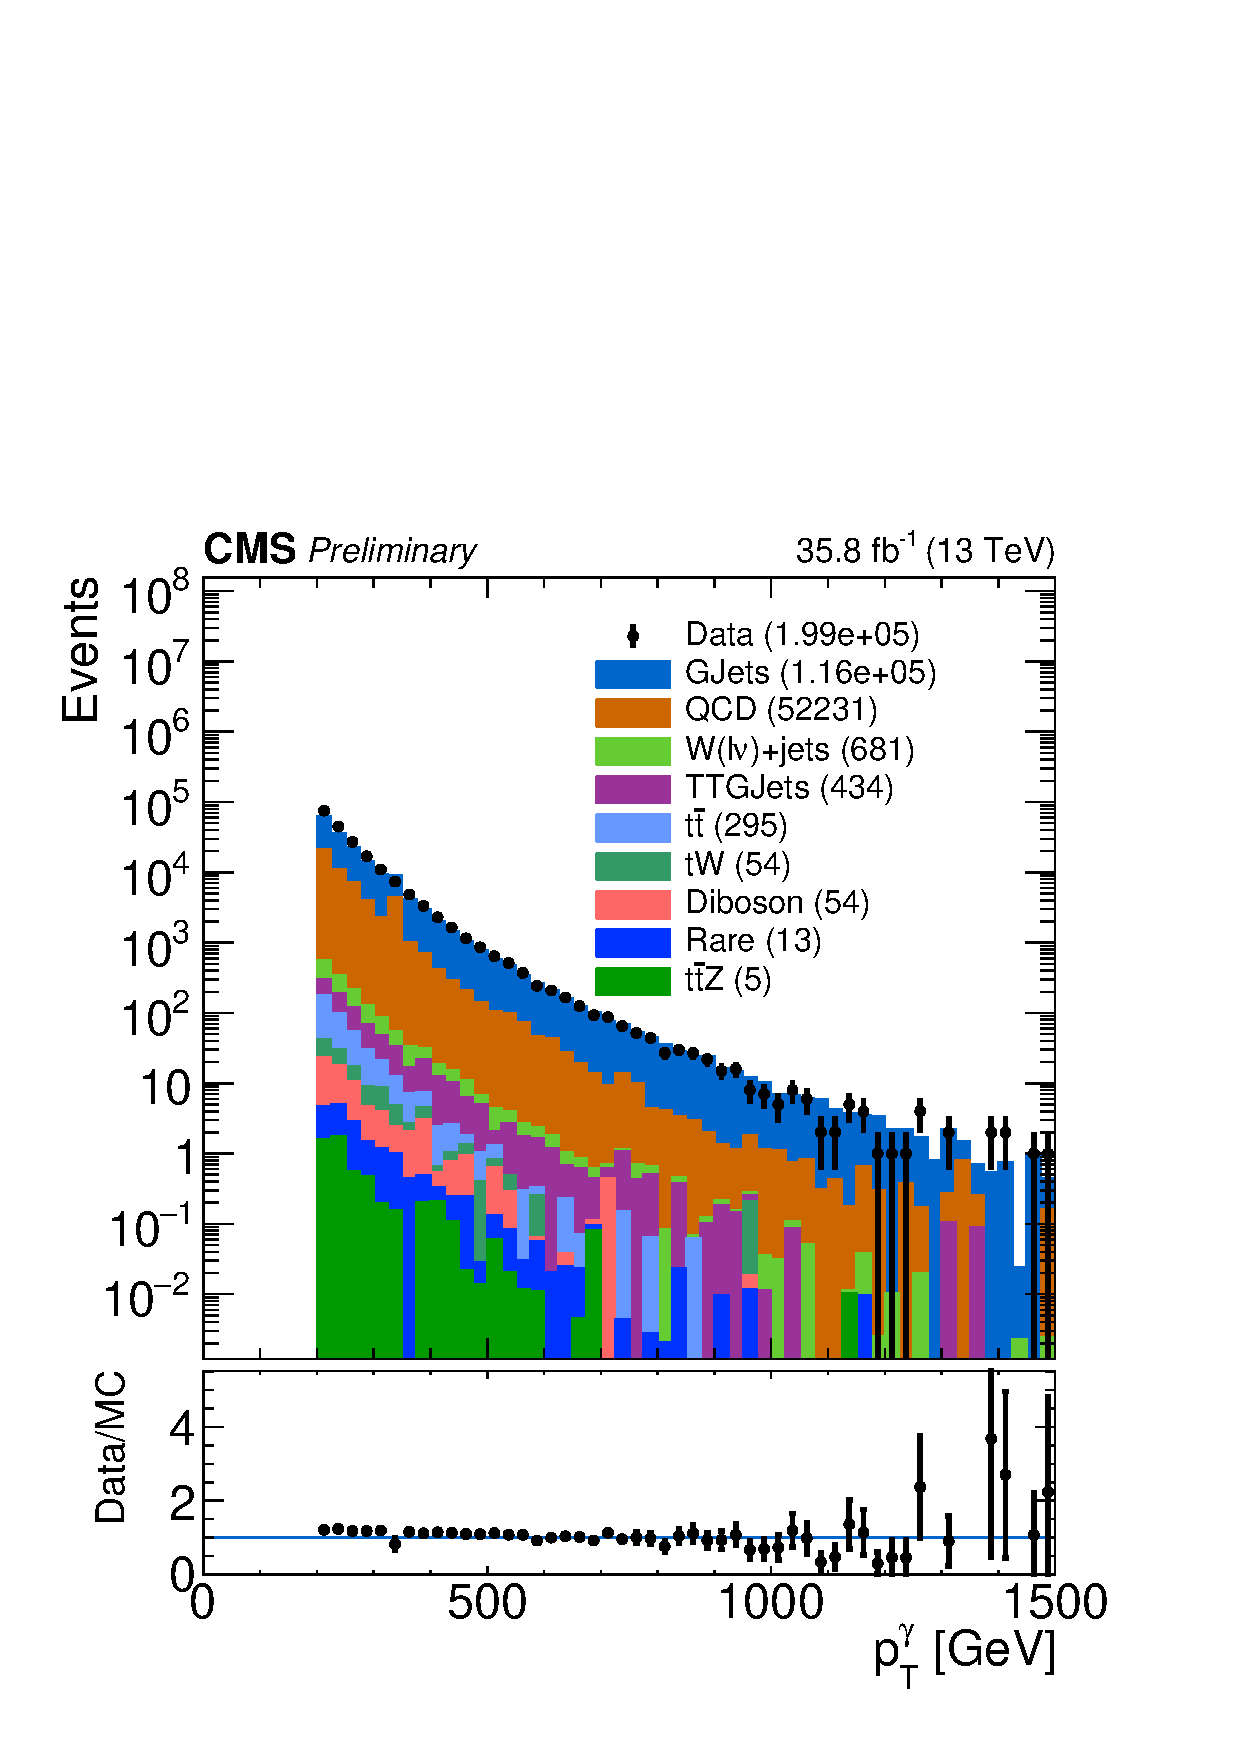
\includegraphics[width=\textwidth]{dataMC_PhotonPt_LooseLepVeto.pdf}
\end{minipage}
\begin{minipage}[b]{0.45\textwidth}
    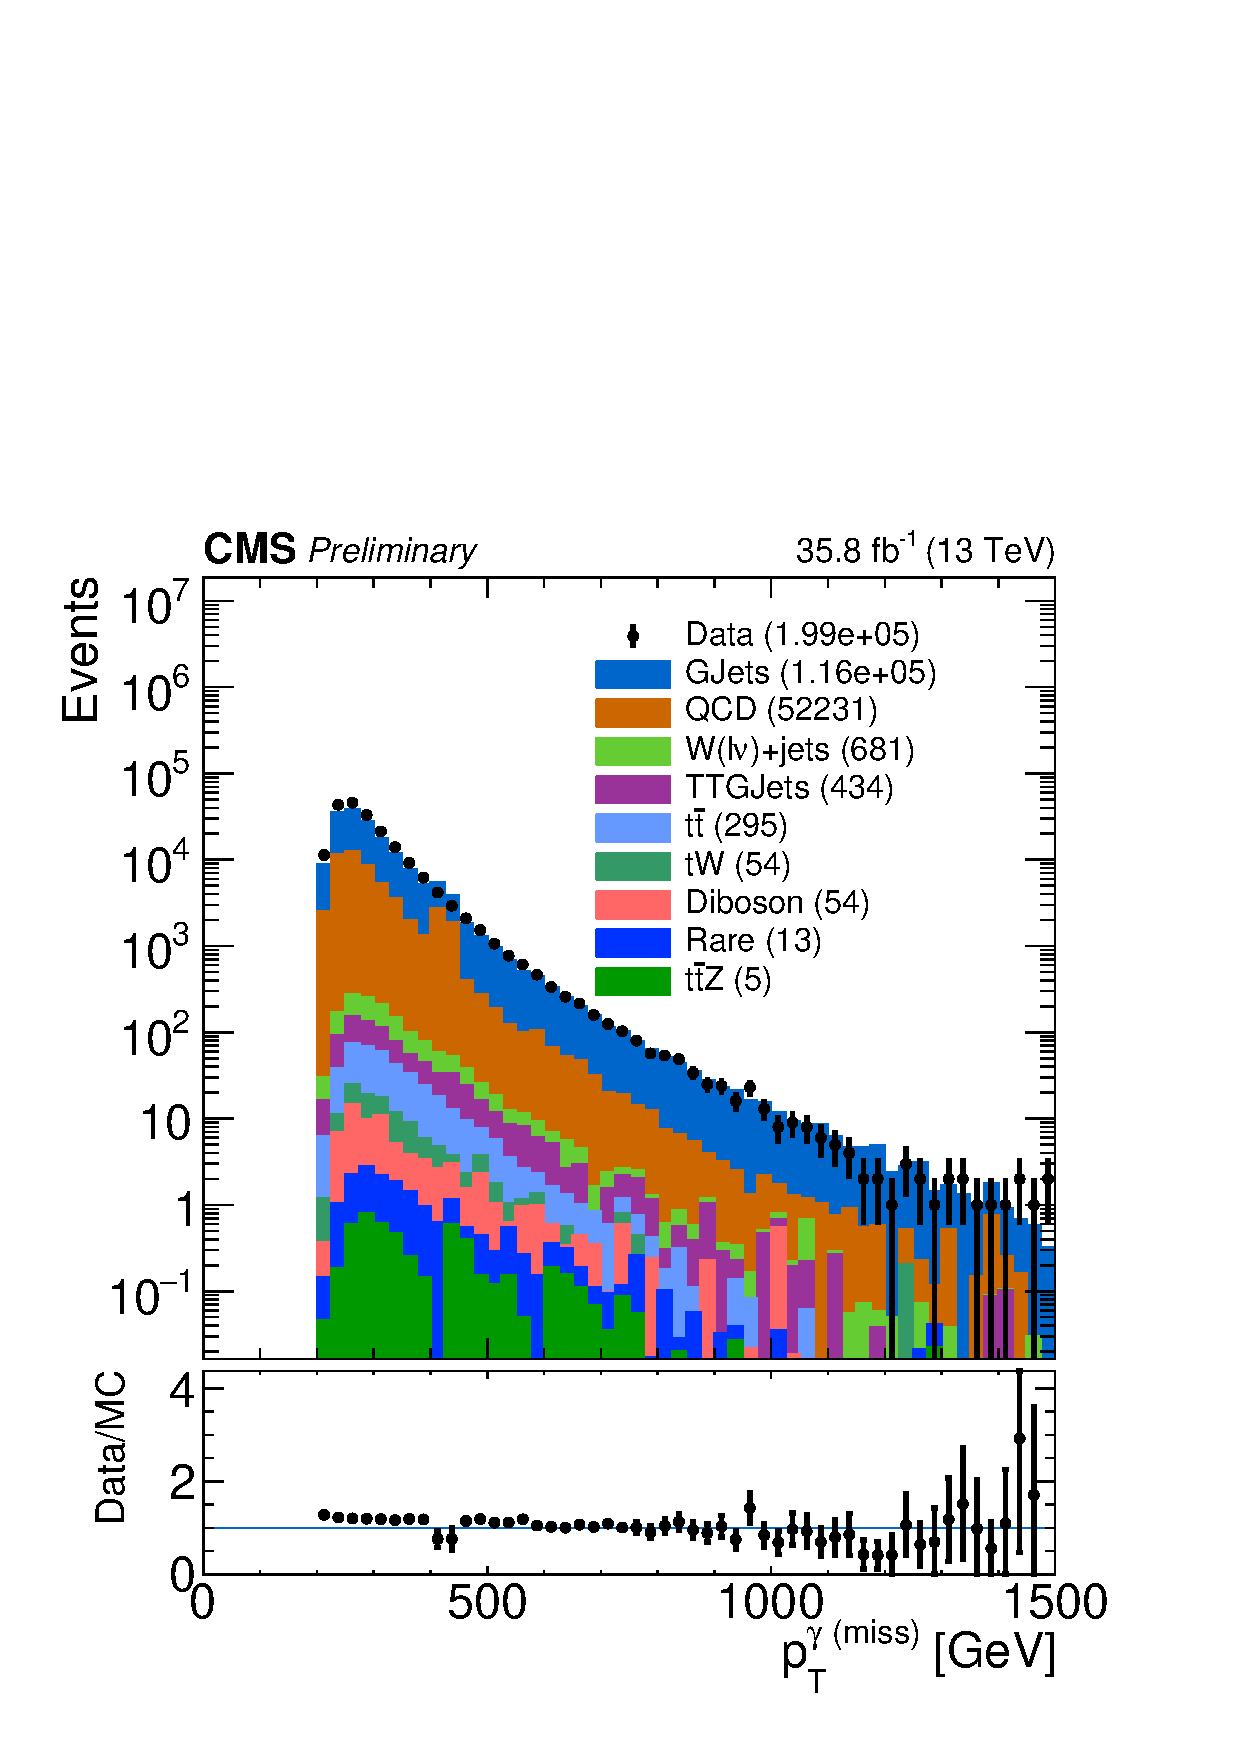
\includegraphics[width=\textwidth]{dataMC_MetGamma_LooseLepVeto.pdf}
\end{minipage}
\end{center}
\vspace{-1em}
\caption{Shown are both the $p_\text{T}^{\gamma}$ (left) and $p_\text{T}^{\gamma (miss)}$ (right) distributions before applying any corrections. $p_\text{T}^{\gamma (miss)}$ is obtained by adding the $p_\text{T}^{\gamma}$ to the total $p_\text{T}^{miss}$ in every event.}
\label{PtMetPt}
\end{figure}
\vspace{1em}

To further emulate the Z$\rightarrow\nu\bar{\nu}$+jets background, a variable in which the photons are treated as $p_\text{T}^{miss}$ is defined. We call this variable $p_\text{T}^{\gamma (miss)}$ and we obtain it by adding the $p_\text{T}^{\gamma}$ for every event to the total $p_\text{T}^{miss}$ in the event. Both the $p_\text{T}^{\gamma}$ and the resulting $p_\text{T}^{\gamma (miss)}$ distributions are shown in \autoref{PtMetPt} as data/MC comparison plots, where the simulated backgrounds are stacked in order of ascending contribution.\\

The main contributions from simulation arise from the $\gamma+$jets, QCD and to a lesser extent, t$\bar{\text{t}}\gamma$. Other non-dominant backgrounds in the control region include contributions from W($l\nu$)+jets, t$\bar{\text{t}}$, Diboson, tW, t$\bar{\text{t}}$Z and rare processes. Most of these lesser backgrounds are nearly negligible (several orders of magnitude lower than the dominant backgrounds) and are considered to be mostly composed of fake photons. In addition to the cuts described, all of the simulation samples are subjected to weights that apply corrections to pileup as well as the b-tagging efficiency. Data, on the other hand, is obtained from a sample that contains events with at least one identified photon. Photons in this sample are also subjected to the high-level trigger HLT\_Photon175, which restricts the selection to photons that have a $p_\text{T} >$ 175 GeV. Both simulation and data are subjected to the same selection criteria established in this section. 

\subsection{Photon Purity and Fake Rate}\label{purity&fakerate}

Three different types of photons make up the $\gamma+$jets CS: prompt photons, produced either directly or through fragmentation, and fake photons. Prompt photons are defined as photons which are formed shortly after the proton-proton collision (i.e. before the produced quarks and gluons have had enough time to form hadrons). Two types of photons fit in this category. The first type, which we designate as direct photons, are photons that are produced directly from the proton-proton interaction\cite{promptPho}. A secondary type of prompt photon, that is virtually indistinguishable from the direct photons at the detector level, originates from the decay of $\pi^0$ mesons and are called fragmentation photons. The final type of photon found in the CS corresponds to fake (or non-prompt) photons. The fake photon contribution typically arises from leptons (mostly electrons) whose tracks are not properly reconstructed, yet leave energy measurements in the ECAL.

\begin{figure}[H]
\begin{center}
\begin{minipage}[b]{0.49\textwidth}
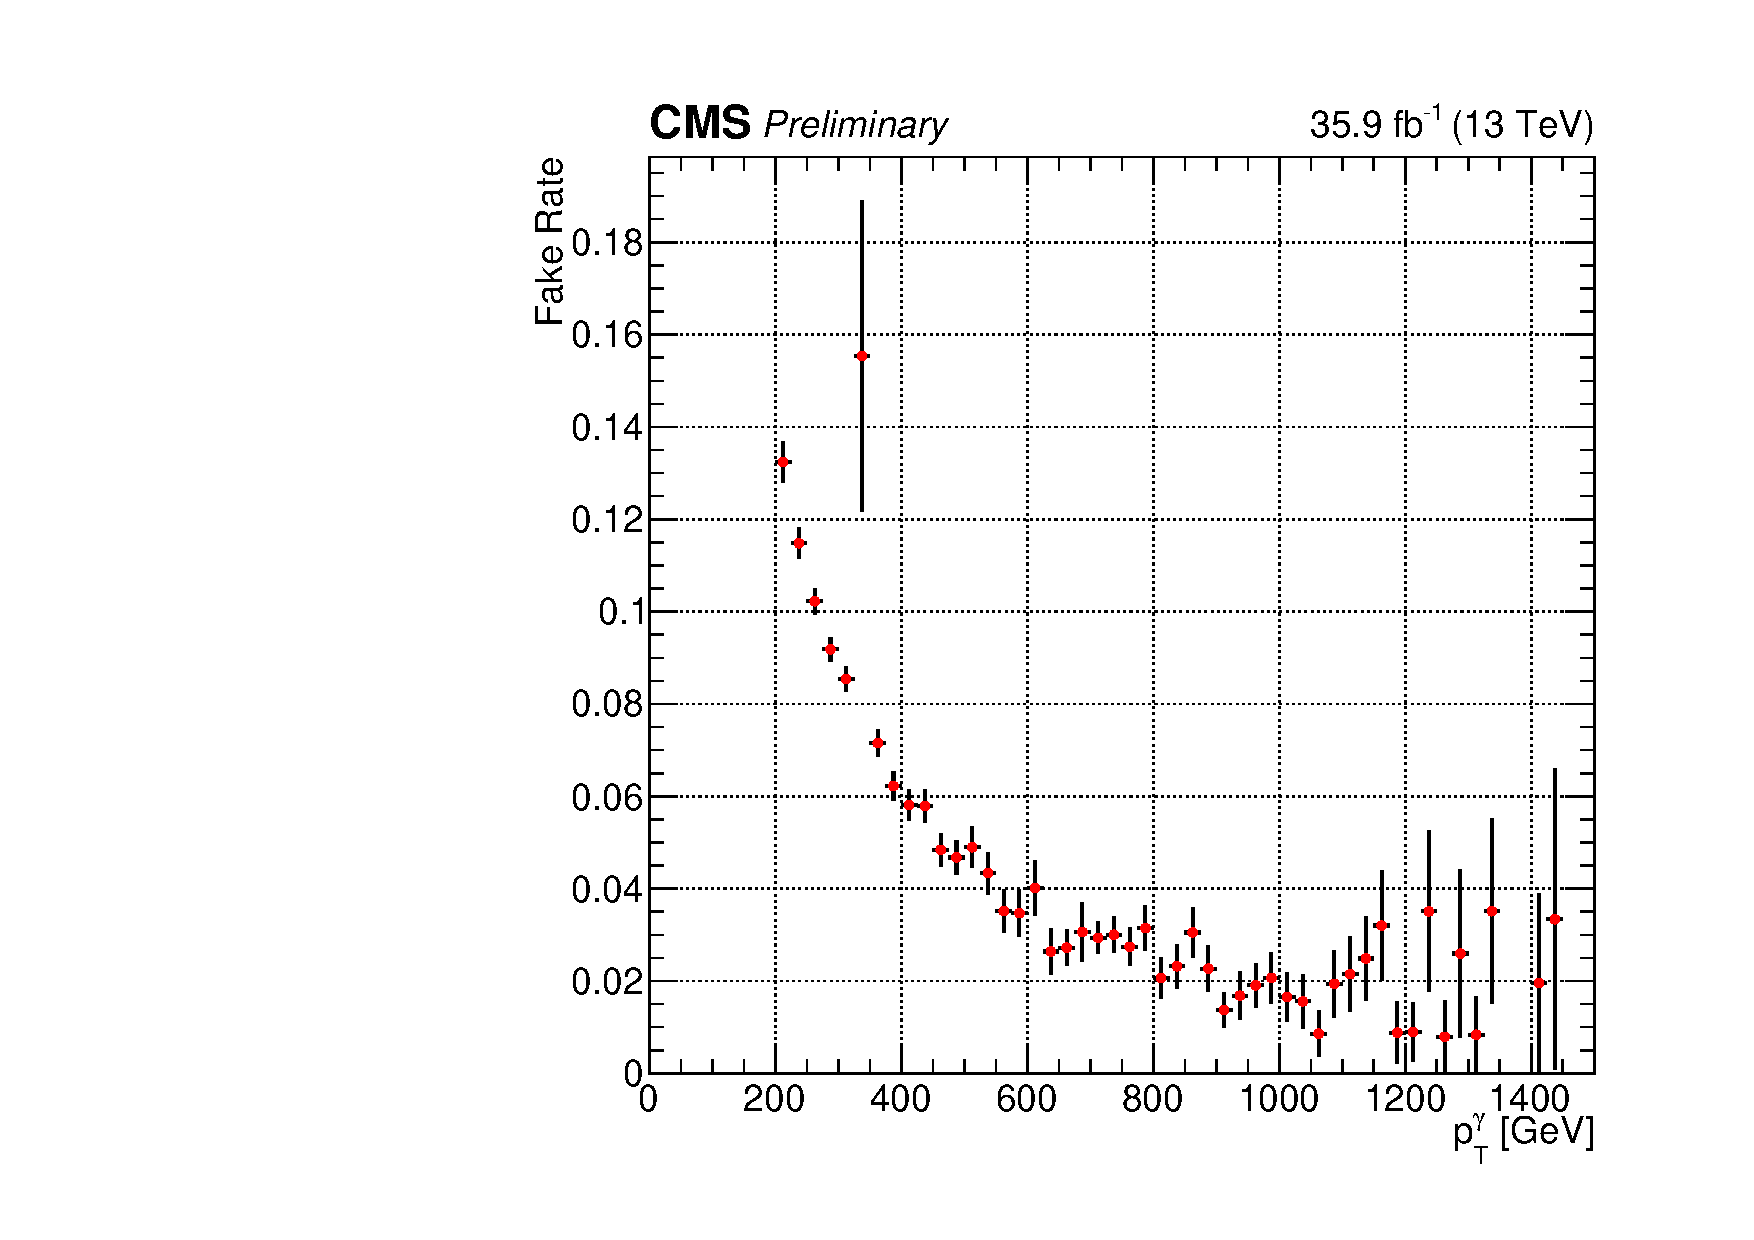
\includegraphics[width=\textwidth]{FakeRate_empty.pdf}
\end{minipage}
\begin{minipage}[b]{0.49\textwidth}
    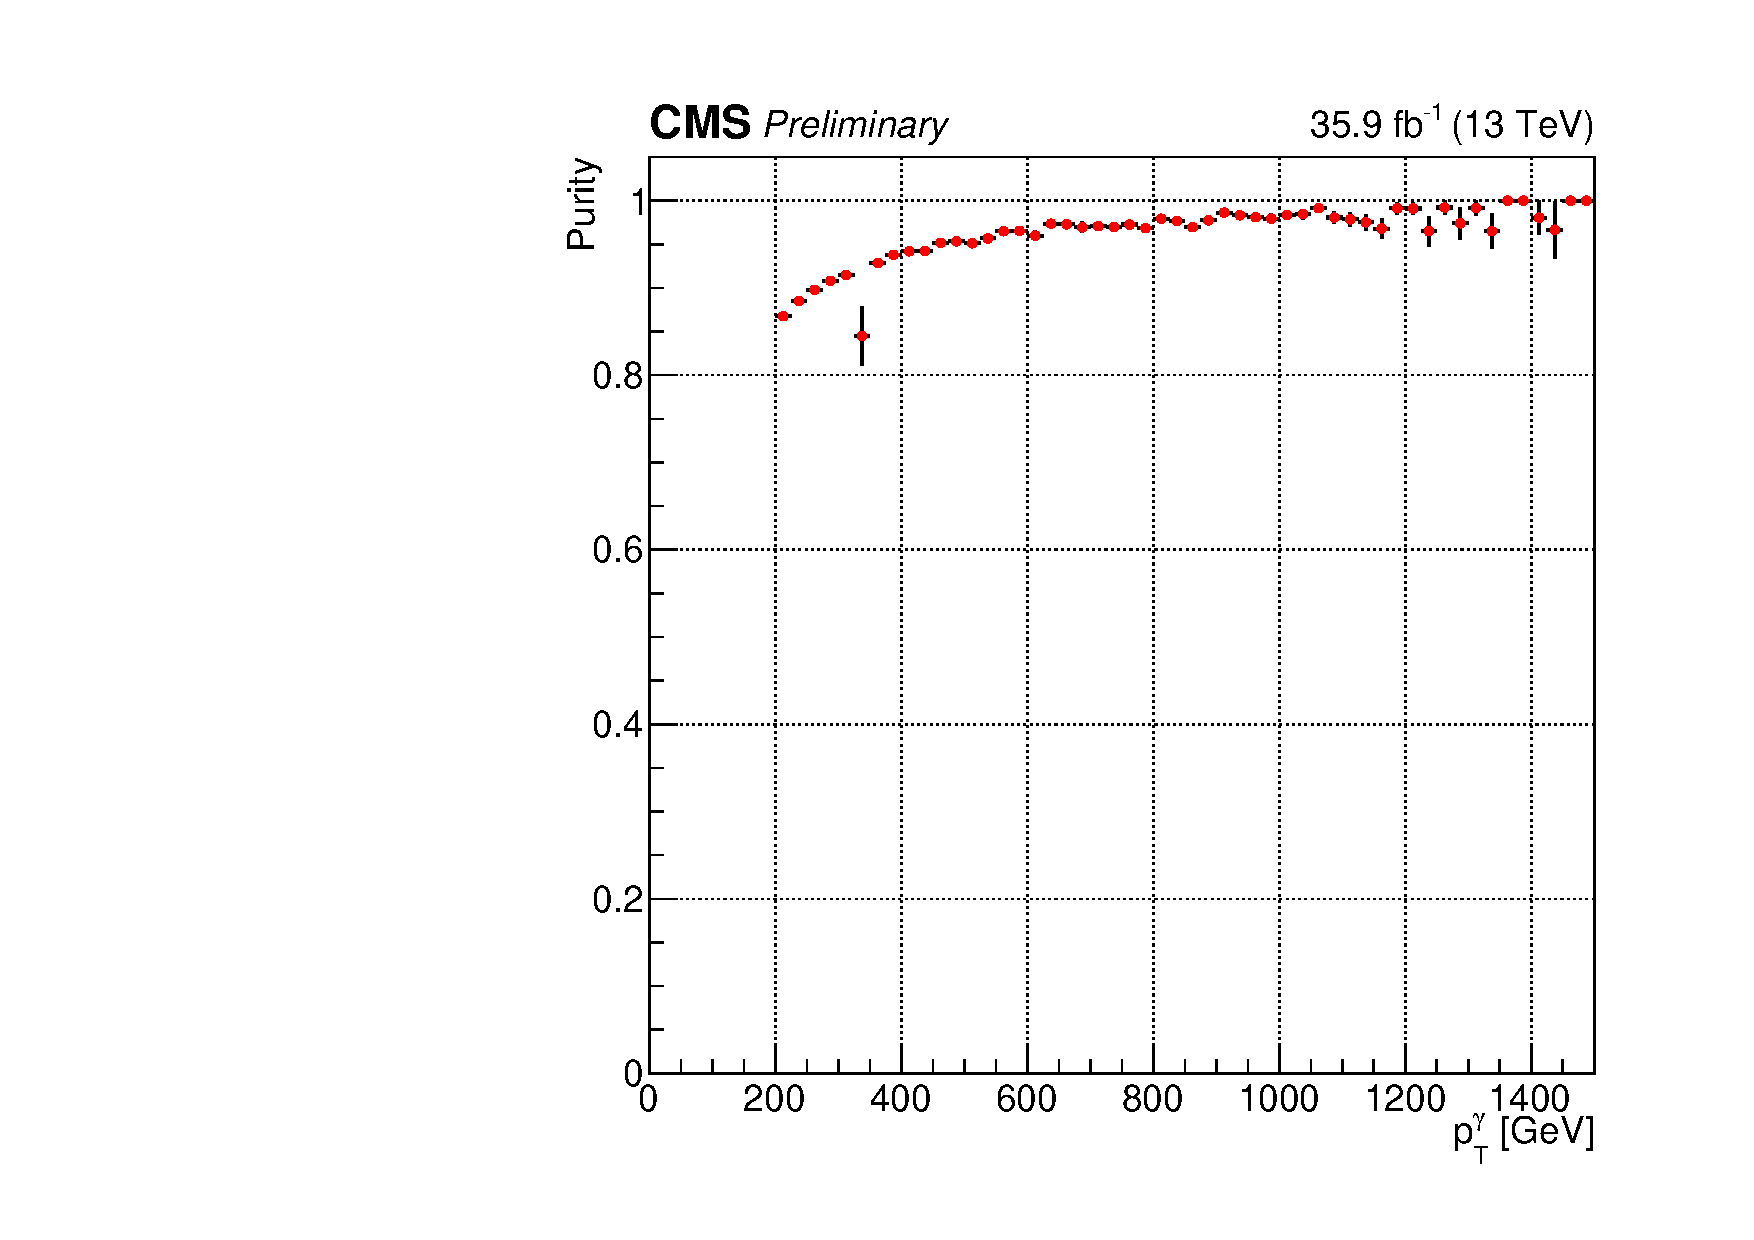
\includegraphics[width=\textwidth]{Purity_empty.pdf}
\end{minipage}
\end{center}
\vspace{-1em}
\caption{Plots for Fake Rate (left) and Purity (right) as a function of the photon $p_\text{T}$ are shown. The events are selected are required to have a $p_\text{T} > 200$ GeV, be within the ECAL acceptance range, and pass the loose ID selection cuts. This selection was produced in order to verify the values given by the E/$\gamma$ POG. As can be seen, the efficiency (purity) is seen to agree with the values of the loose photon ID/isolation selection.}
\label{FakeRatePurityLoose}
\end{figure}

\begin{figure}[H]
\begin{center}
\begin{minipage}[b]{0.49\textwidth}
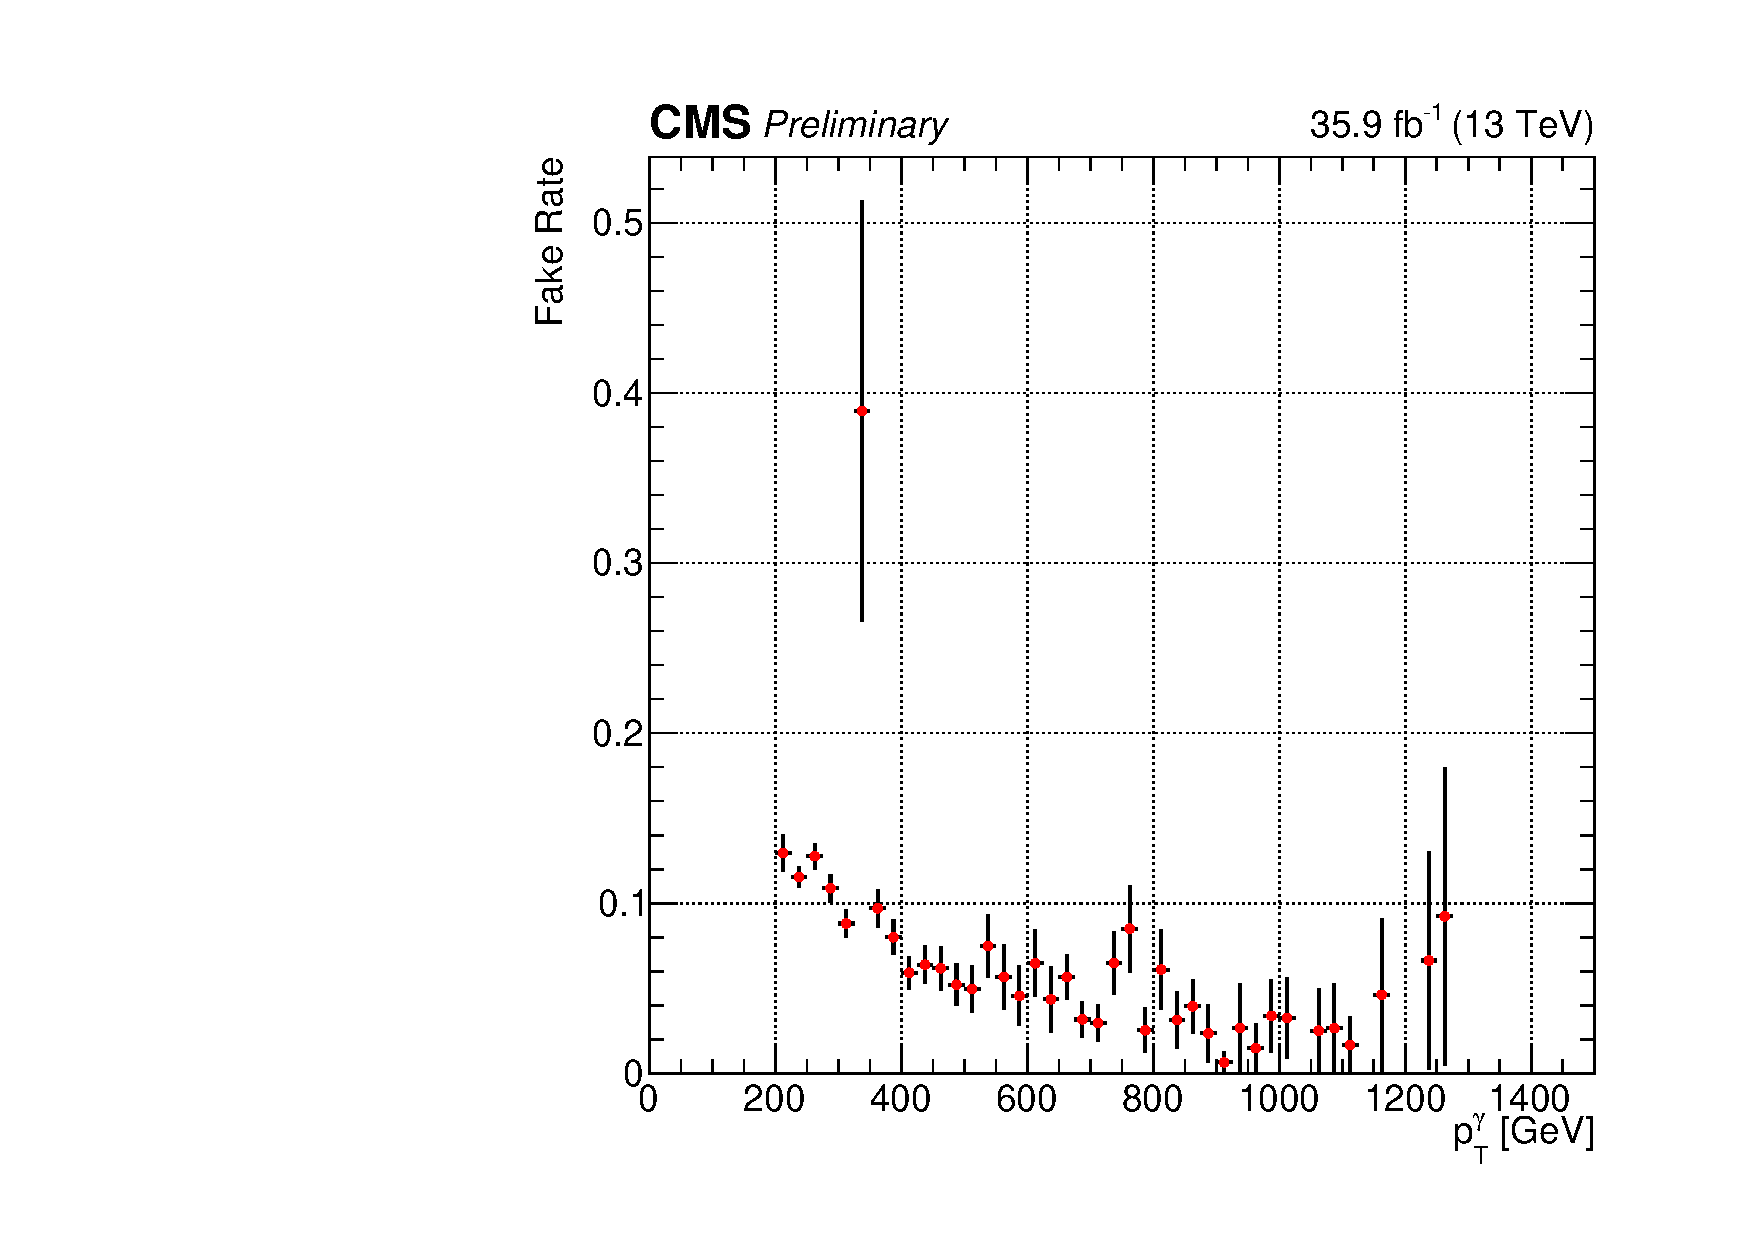
\includegraphics[width=\textwidth]{FakeRate_LooseLepVeto.pdf}
\end{minipage}
\begin{minipage}[b]{0.49\textwidth}
    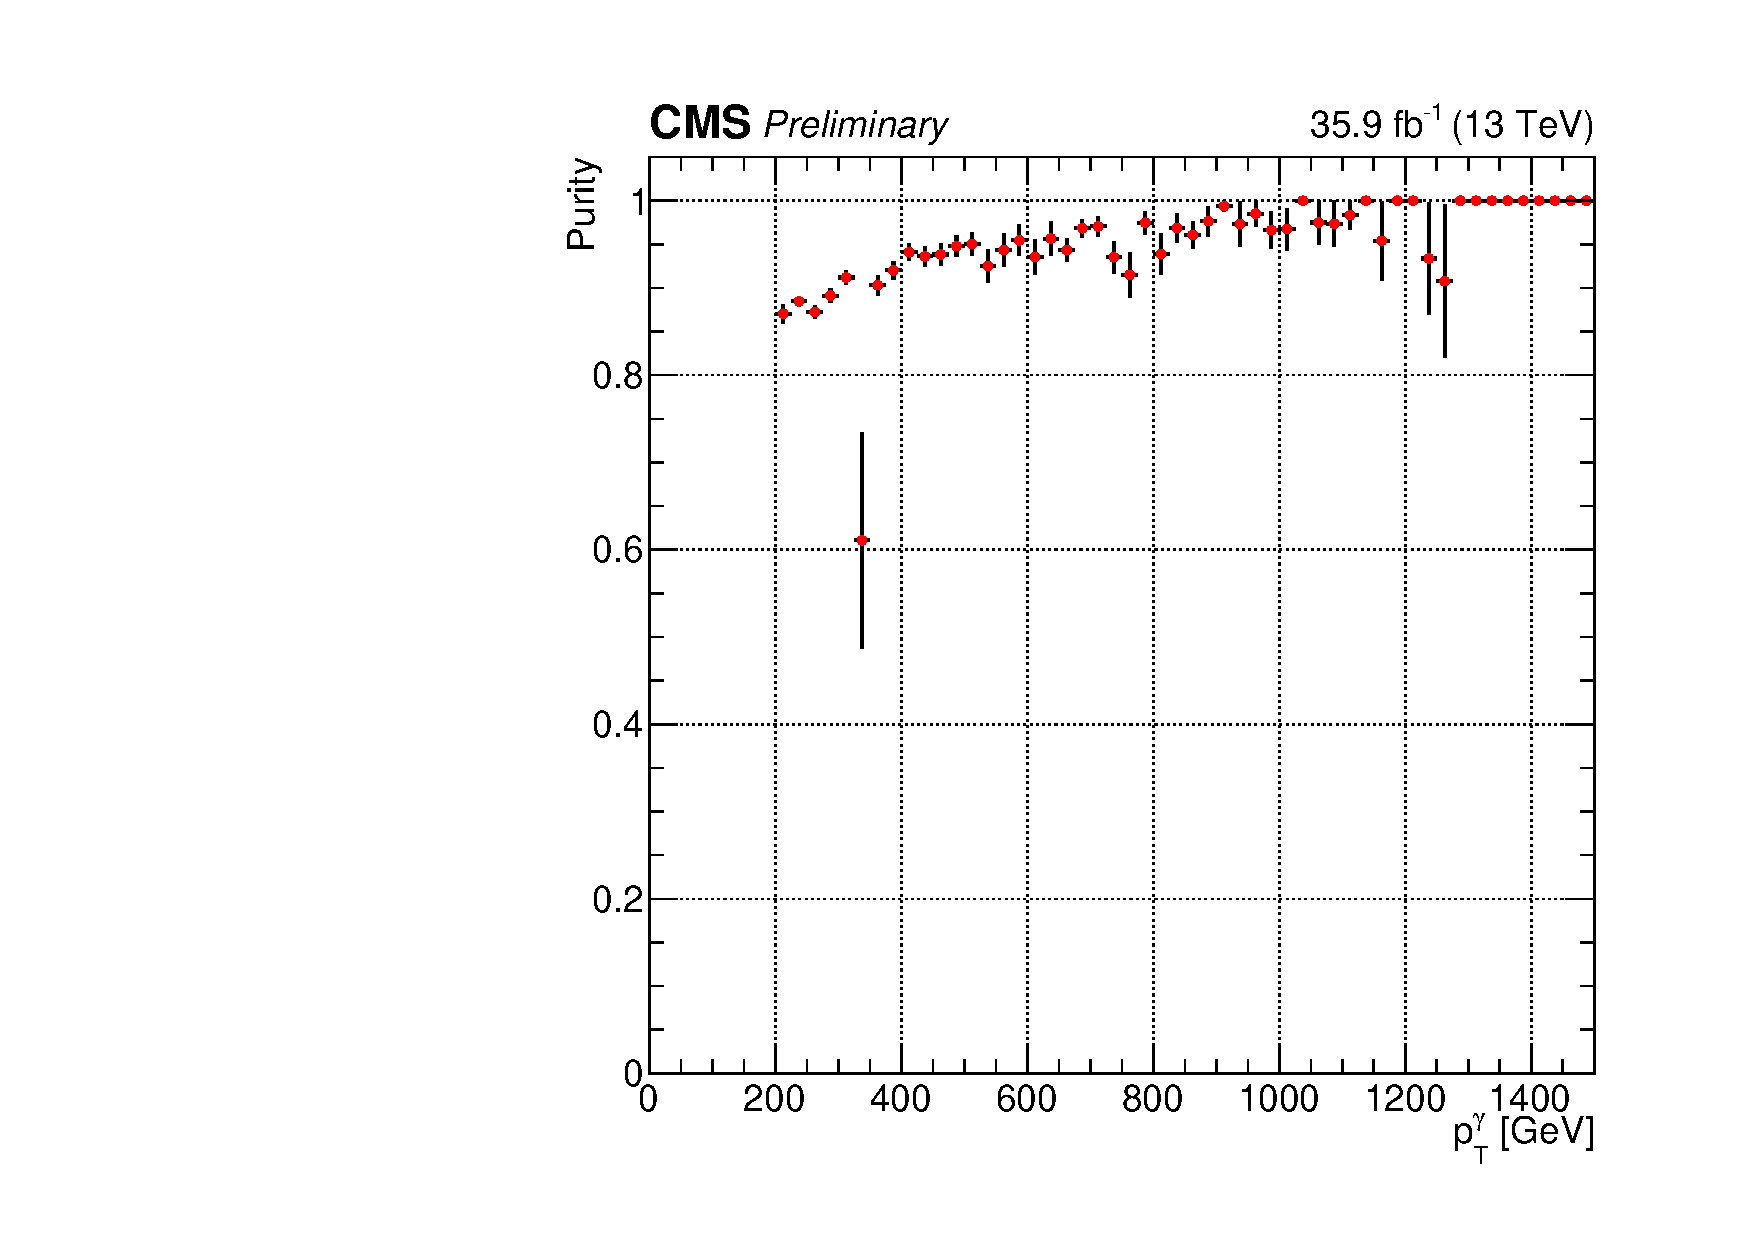
\includegraphics[width=\textwidth]{Purity_LooseLepVeto.pdf}
\end{minipage}
\end{center}
\vspace{-1em}
\caption{Plots for Fake Rate (left) and Purity (right) as a function of the photon $p_\text{T}$ are shown. These plots include photons with the full control region selection. Aside from exhibiting lower statistics, the plots seem to agree with the fake rate and purity before all the control region cuts are applied.}
\label{FakeRatePurityCR}
\end{figure}

\vspace{1em}

In order to identify prompt photons, reconstructed photons from the $\gamma+$jets and QCD samples are matched to generator-level photons in space and momentum by requiring $\Delta R(\gamma_\text{gen},\gamma_\text{reco}) < 0.4$ and $0.5 < p_\text{T}^\text{gen}/p_\text{T}^\text{reco} < 2.0$, respectively. Any reconstructed photon which fails to get matched to a generator level photon is labeled as a fake/non-prompt photon. Direct photons are identified by further requiring that the reconstructed photons be matched to a parton (a gluon or quark) in space as $\Delta R(\gamma,\text{parton}) > 0.4$. This requirement is intended to distinguish the reconstructed photons from highly boosted $\pi^0$'s, which compose a large portion of the experimentally indistinguishable fragmentation photons. Finally, fragmentation photons are obtained exclusively from QCD simulation and are required to have $\Delta R(\gamma,\text{parton}) < 0.4$ in order to avoid double counting photons from the $\gamma+$jets sample.\\

With all three types of photons defined, a study can be carried out from simulation to estimate their respective contributions to the defined control region. The study takes into account that any reconstructed photon in the $\gamma+$jets or QCD samples can only be categorized as prompt (through direct production or fragmentation) or non-prompt (fake). The purity and fake rate can then be defined in terms of the relative proportions of prompt or non-prompt photons with respect to the sum of the contributions from all three types of photons. Identified direct photons are taken from the $\gamma+$jets sample exclusively. Meanwhile, the fragmentation and fake photon contributions are taken from the QCD sample. The three quantities are then added together and their respective contributions are determined in terms of the photon $p_\text{T}$ (\autoref{FakeRatePurityLoose}).\\

The photon purity (\autoref{FakeRatePurityLoose} and \autoref{FakeRatePurityCR}, right) is defined in terms of the prompt and non-prompt photons as:\\

\begingroup
	\large
	\begin{center}
	%\begin{equation}
		$p_\gamma = \frac{prompt}{prompt+fake}$ ,
	\end{center}
	%\end{equation}
\endgroup
\vspace{1em}

\noindent{where the prompt photon portion comes from the sum of the direct photons (extracted from the $\gamma$+ jets sample) and the fragmentation photons (extracted from the QCD sample). The remaining non-prompt (or fake) photons all come from photons in the QCD sample that were not matched to truth-level photons in space and momentum with the specified required conditions. Meanwhile, the photon fake rate (\autoref{FakeRatePurityLoose} and \autoref{FakeRatePurityCR}, left) is defined from this same combination of samples as:}\\

\begingroup
	\large
	\begin{center}
	%\begin{equation}
		$f = \frac{fake}{prompt+fake}$ ,
	\end{center}
	%\end{equation}
\endgroup
\vspace{1em}

\autoref{FakeRatePurityLoose} shows the purity and fakerate for photons that pass the loose ID/selection, have a $p_\text{T} > 200$ GeV and are within the ECAL acceptance range. A sample is obtained in which 77\% of the photons are direct, 12\% are fragmentation and 11\% are fakes. This implies an average purity of $\sim$89\% for this sample, well within the value that is expected. \autoref{FakeRatePurityCR} shows the same ratios for the loose $\gamma$+ jets control region described in \autoref{photonSelection}. Although the amount of statistics has decreased due to the additional cuts, a similar trend can be observed.

\section{The Z$\rightarrow\mu^{+}\mu^{-}$ Control Region}

The Z$\rightarrow\mu^{+}\mu^{-}$ control region defined in this section is in every respect identical to the one applied in the 2016 analysis (\autoref{ZnunuSection}. The only difference between the 2016 method and the one discussed in this chapter is that the Drell-Yan (DY) sample is only used for the normalization correction of the Z$\rightarrow\nu\bar{\nu}$ background. Therefore, the loose $\mu\mu$ control region is not used or applied in the calculation of the scale factors. In the following subsections only the tight $\mu\mu$ control region, and its usage to obtain the normalization scale factor $R_{norm}$, is discussed.

\subsection{Muon ID and Isolation}

The muons are selected using the ``medium muon'' selection\cite{muonID}, per the recommendation of the muon POG. The muon candidates in this selection satisfy $p_\text{T} > 10$ GeV and $|\eta| < 2.4$. Other additional cuts are applied to aid in the muon candidate selection, such as an impact parameter cut. Muons are also subjected to a PF relative-isolation (also referred to as mini-isolation) in which the cone size is inversely proportional to the muon $p_\text{T}$. This requirement enforces the $p_\text{T}$ within the isolation cone to be at most 20\% of the muon $p_\text{T}$ in order to eliminate events with an isolated muon. Details of the medium photon selection are included in \autoref{table1muons} and \autoref{table2muons}, while details of the impact parameter cut are summarized in \autoref{table3muons}.

\begin{table}[H]
\begin{center}
\includegraphics[width=0.6\textwidth]{table1muons}
\caption{Muon Medium ID 2016 HIP Safe}
\label{table1muons}
\end{center}
\end{table}

\begin{table}[H]
\begin{center}
\includegraphics[width=0.4\textwidth]{table2muons}
\caption{Muon Medium ID HIP Safe Good Global Muon}
\label{table2muons}
\end{center}
\end{table}

\begin{table}[H]
\begin{center}
\includegraphics[width=0.3\textwidth]{table3muons}
\caption{Additional Impact Parameter cut on Muons}
\label{table3muons}
\end{center}
\end{table}

\subsection{Muon Selection in the Tight Control Region}\label{tightmumu}

Events are selected from data samples that contain exactly two oppositely charged muons ($\mu^{+}\mu^{-}$), which fall within the invariant mass $81 < m_{ll} < 101$ GeV window for the Z boson. Additional cuts for the tight muon selection include baseline requirements such as an $H_\text{T} > 300$ GeV, $N_j \geq 4$, the $\Delta\phi$ baseline cut on leading jets, a $p_\text{T}^{miss} > 250$ GeV, an $m_\text{T2} > 200$ GeV and at least 1 top-tagged jet $N_t \geq 1$. In addition, the $p_\text{T}$ of the two muons are required to be $p_\text{T} > 50$ GeV for the leading muon and $p_\text{T} > 20$ GeV for the sub-leading one. The only difference, when compared to the signal region is the missing lepton veto, in addition to the dimuon events being treated as $p_\text{T}^{miss}$. This makes for a region that exhibits very similar kinematics to the Z$\rightarrow\nu\bar{\nu}$ signal region, yet suffers from a lack of statistics.

\section{Analysis}

In this section a detailed explanation of the calculation of the scale factors for both shape and normalization corrections is provided. The following methods make use of the loose $\gamma+$jets and the tight $\mu\mu$ control regions defined in the previous sections. The procedure involves extracting the shape corrections $S_\gamma$ from the $\gamma+$jets control region and afterwards obtain a single normalization correction factor $R_{norm}$ from the tight $\mu\mu$ control region. Both factors will then be applied to the final prediction of the Z$\rightarrow\nu\bar{\nu}$ background in each of the required search bins. 

\subsection{Shape Correction Using the $\gamma$ + jets Control Sample}

In this section the validation of the $\gamma+$jets simulation is discussed in terms of the shape of the loose photon control region. As it was shown in \autoref{purity&fakerate}, this control region has high purity for $\gamma+$jets events, particularly in regions of high $p_\text{T}$ ($\gtrsim 300$). In order to apply this correction factor it is assumed that the shape differences between data and simulation are similar between Z$\rightarrow\nu\bar{\nu}$ and $\gamma+$jets events. This assumption is validated in studies which compare the cross-section ratio of Z+jets to $\gamma+$jets events\cite{ZtoGamma}. \autoref{Zgamma} shows the results of this study, conducted in 2014, for both data and MadGraph simulation with an integrated luminosity of 19.7fb$^{-1}$ and a center-of-mass energy of 8 TeV. It can be seen that for values of $p_\text{T}^{Z/\gamma} \gtrsim 300$ GeV, the ratio of the cross-section of both processes becomes nearly constant. It is then a matter of applying a factor to account for the difference in the amount of events between the Z+jets and $\gamma+$jets events in order to obtain the total amount of Z$\rightarrow\nu\bar{\nu}$+jets events. This factor is obtained from the tight $\mu\mu$ control region, as shown in \autoref{tightmumu}.

\begin{figure}[H]
\begin{center}
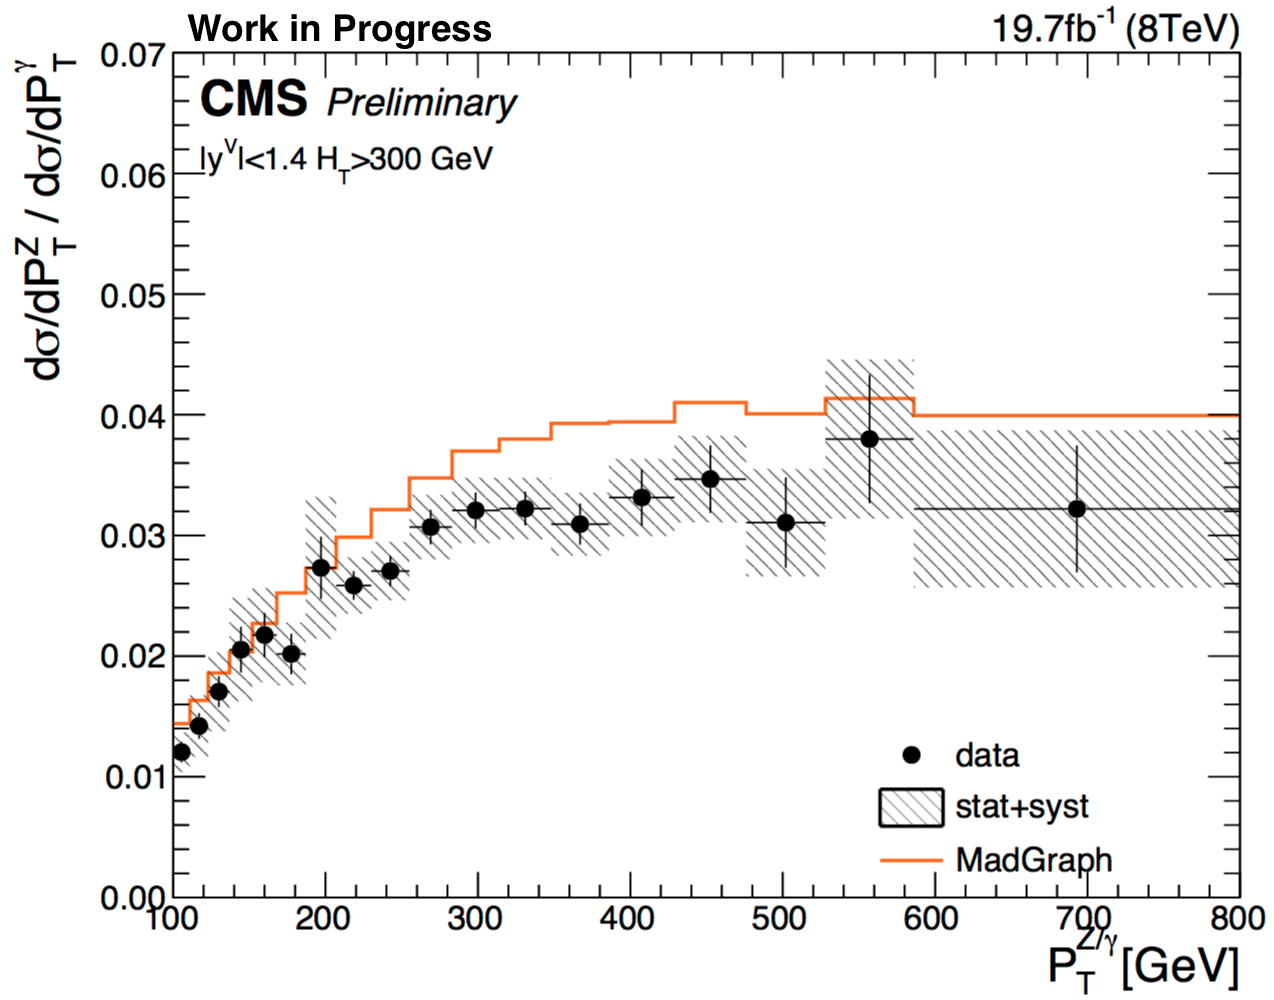
\includegraphics[width=0.6\textwidth]{ZgammaRatio.png}
\end{center}
\vspace{-1em}
\caption[Results of study of the Z+jets to $\gamma+$jets cross-section ratio for both data and MadGraph simulation.]{Results of study of the Z+jets to $\gamma+$jets cross-section ratio for both data and MadGraph simulation. For high values of the vector boson transverse momentum, the ratio between these processes is observed to be nearly constant.}
\label{Zgamma}
\end{figure}

\vspace{1em}

In order to obtain the shape corrections, the ratio between data and simulation of the jet multiplicity distribution is used (\autoref{NjetsCR}). This is due to it exhibiting the highest difference between the observed data and MC. The re-weight for the $\gamma+$jets simulation sample is then accomplished by applying the $N_{jet}$ dependent factor $S_\gamma(N_j)$. This scale factor is determined by taking the ratio of the data and simulation, after subtracting all other MC samples from data events:

\begingroup
	\Large
	\begin{center}
	%\begin{equation}
		$S^{i}_{\gamma} = \frac{\text{Data}^{i} - \text{M}\text{C}^{i}_\text{other}}{\text{M}\text{C}_{\gamma+\text{jets}}^i}$,
	\end{center}
	%\end{equation}
\endgroup

\noindent {where i denotes any given bin in the $N_j$ distribution. The shape correction factors $S^{i}_{\gamma}$ are displayed graphically in \autoref{NjetsCR} (right) for each $N_j$ bin. These factors correct for differences in the jet multiplicity shape, while the overall normalization is estimated from the tight $\mu\mu$ control region. \autoref{NjetsShapeCorr} shows the $N_j$ distribution in the tight $\mu\mu$ control region after the calculated scale factors have been applied. The $S_{\gamma}$ correction will be applied to the Z$\rightarrow\nu\bar{\nu}$ simulation final prediction for each of the analysis search bins. The uncertainty associated with the scale factor is estimated from the event yields in the loose photon control region. This uncertainty will form part of the total systematic uncertainty in the final prediction.}

\begin{figure}[H]
\begin{center}
\begin{minipage}[b]{0.45\textwidth}
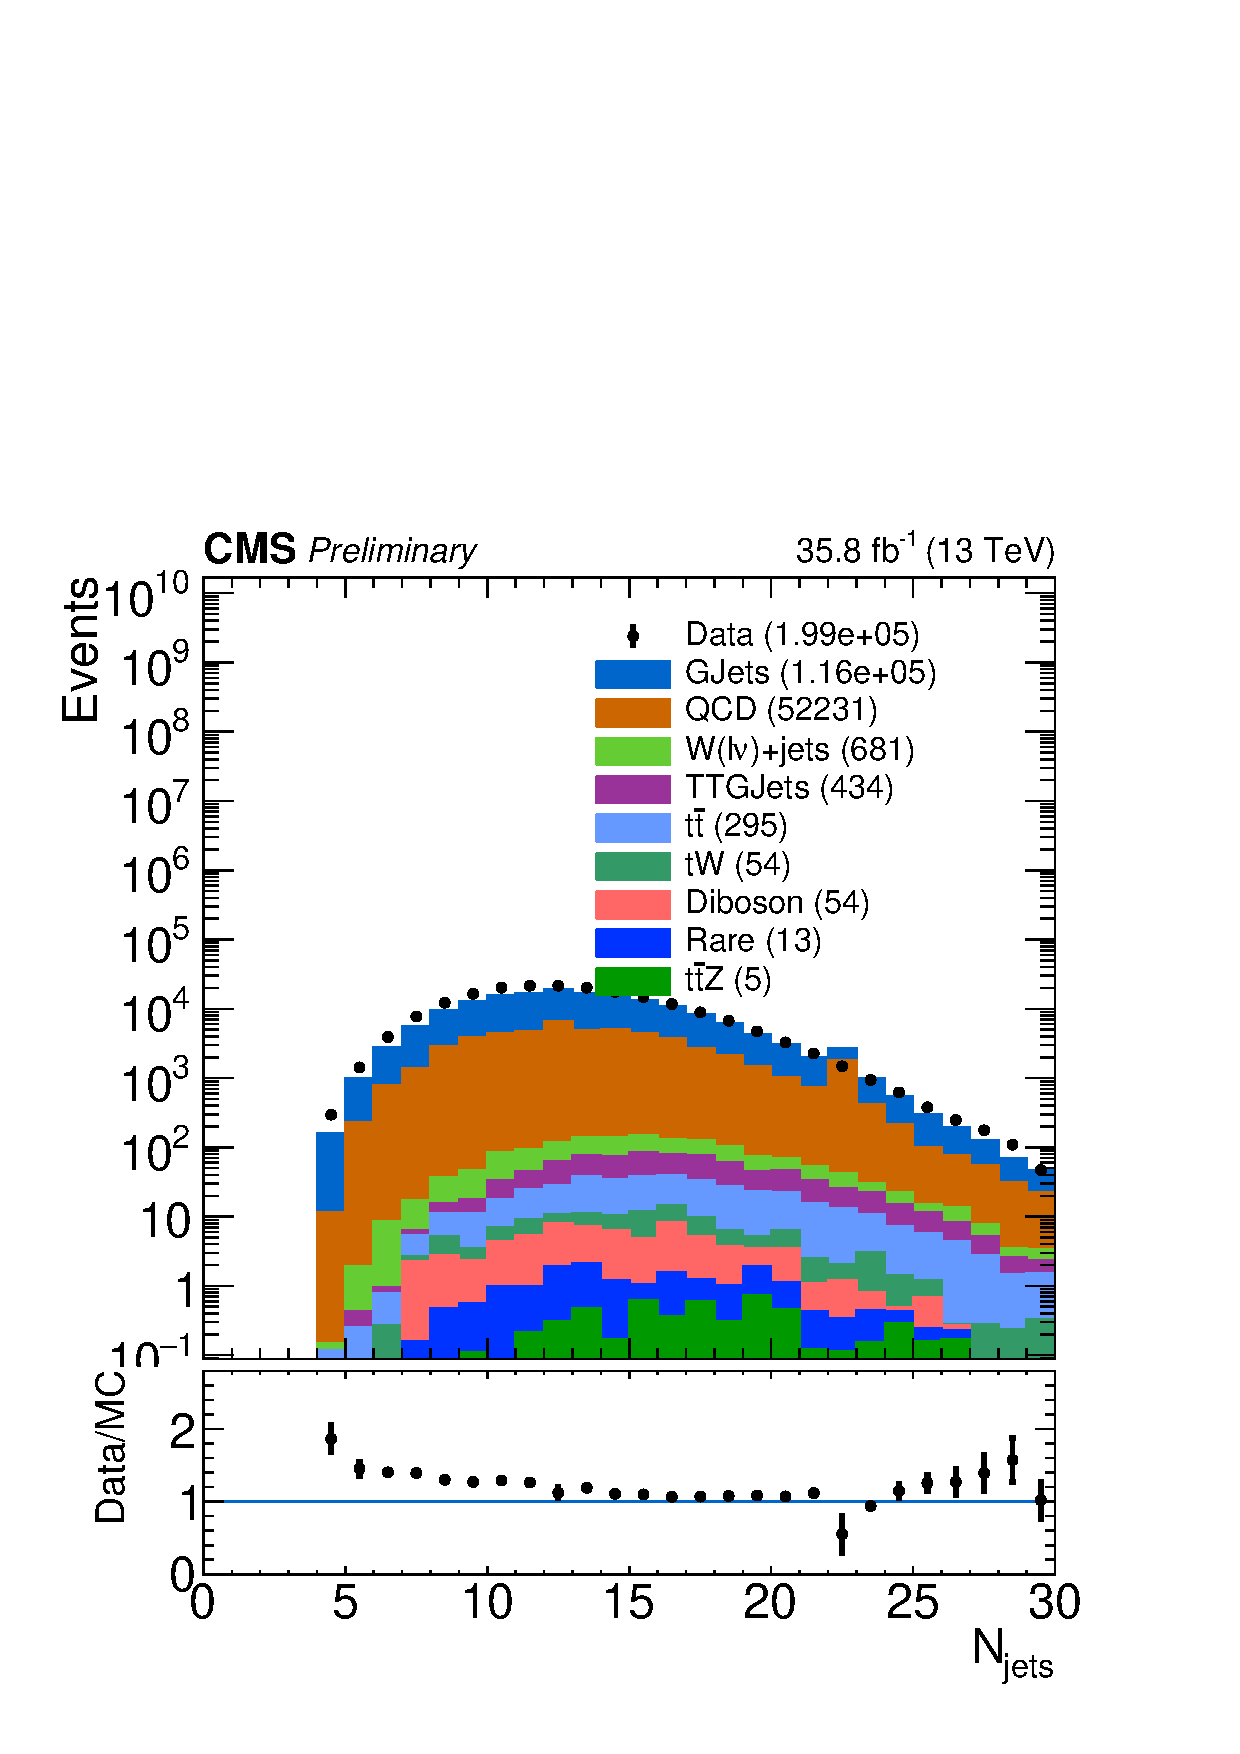
\includegraphics[width=0.94\textwidth]{dataMC_Photon_nj_Log_LooseLepVeto.pdf}
\end{minipage}
\begin{minipage}[b]{0.5\textwidth}
    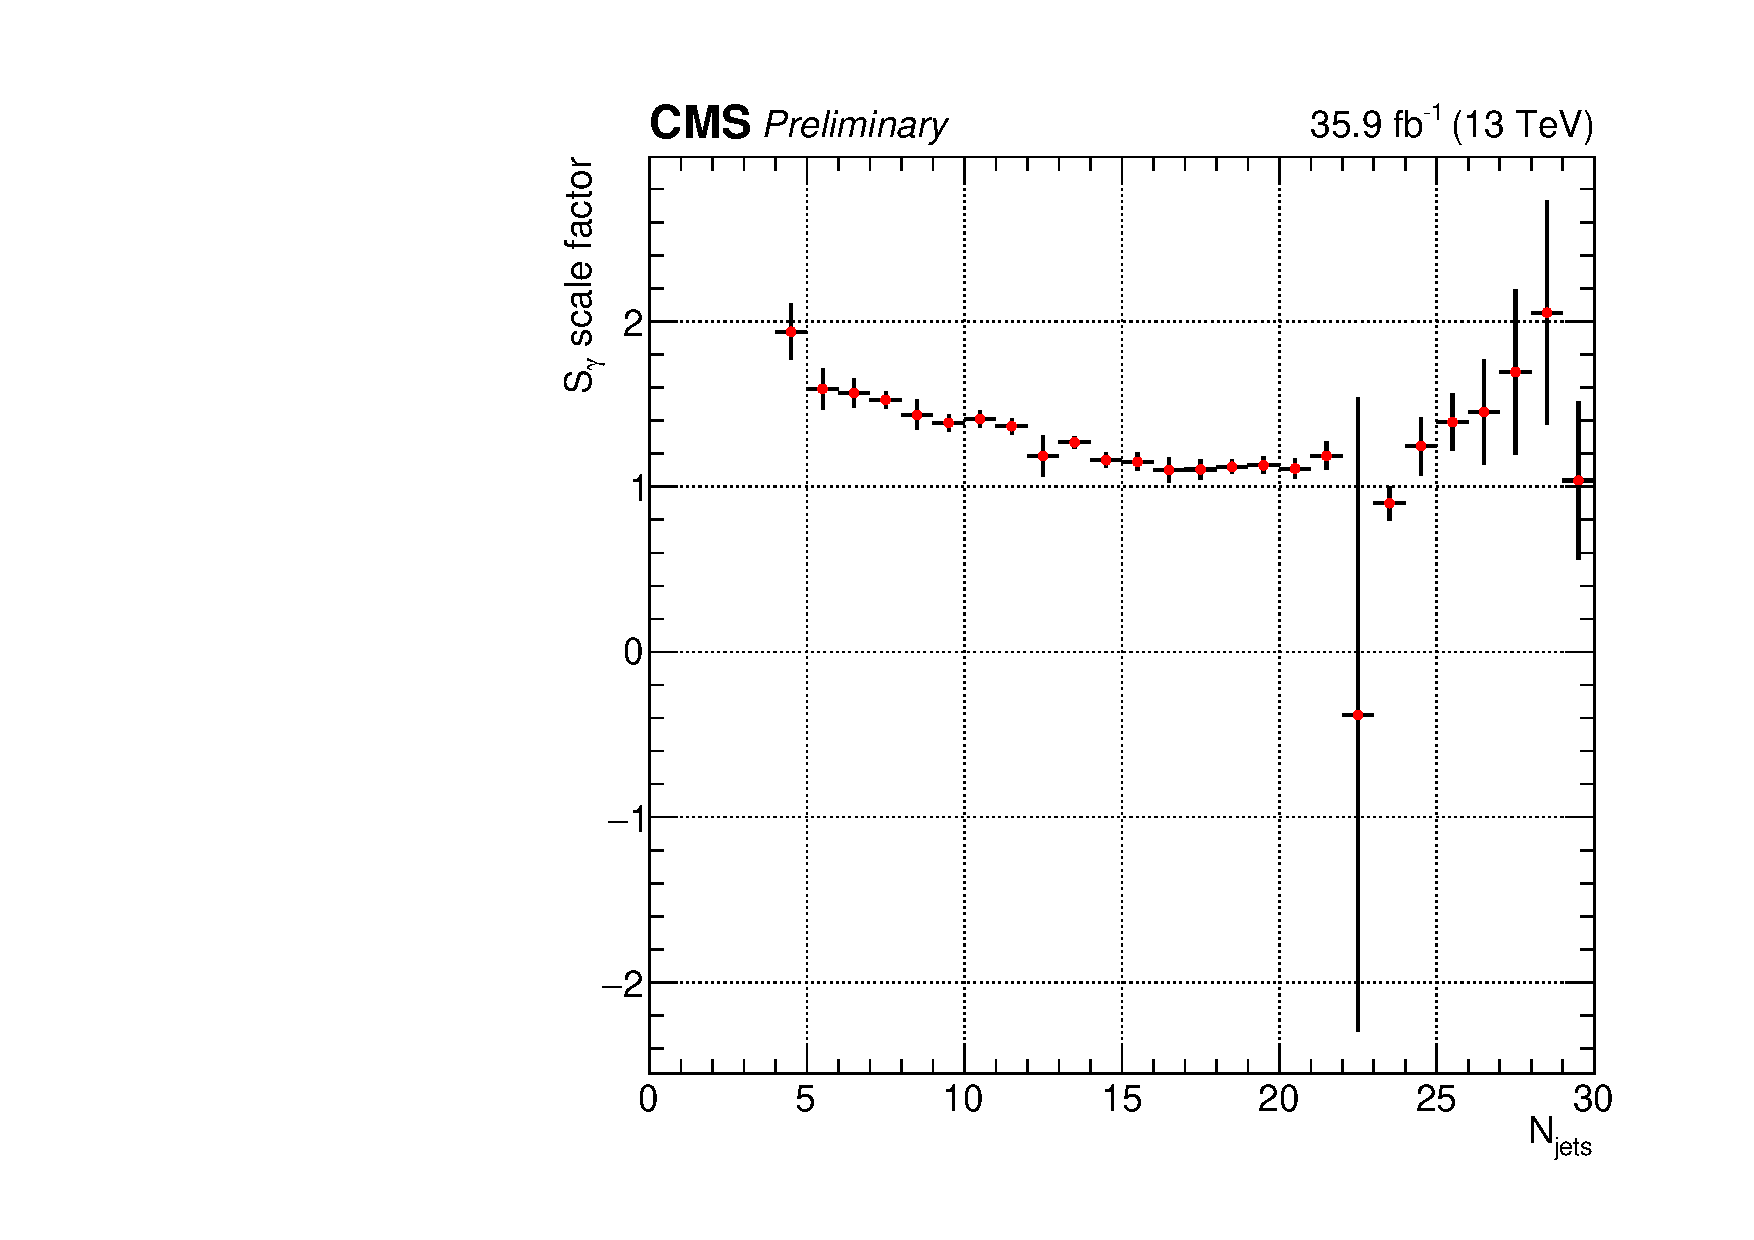
\includegraphics[width=\textwidth]{ShapeCorr_LooseLepVeto.pdf}
\end{minipage}
\end{center}
\vspace{-1em}
\caption{Jet multiplicity and the associated S$_\gamma$ scale factor in the loose photon control region before any corrections are applied.}
\label{NjetsCR}
\end{figure}

%\vspace{1em}

\begin{figure}[H]
\begin{center}
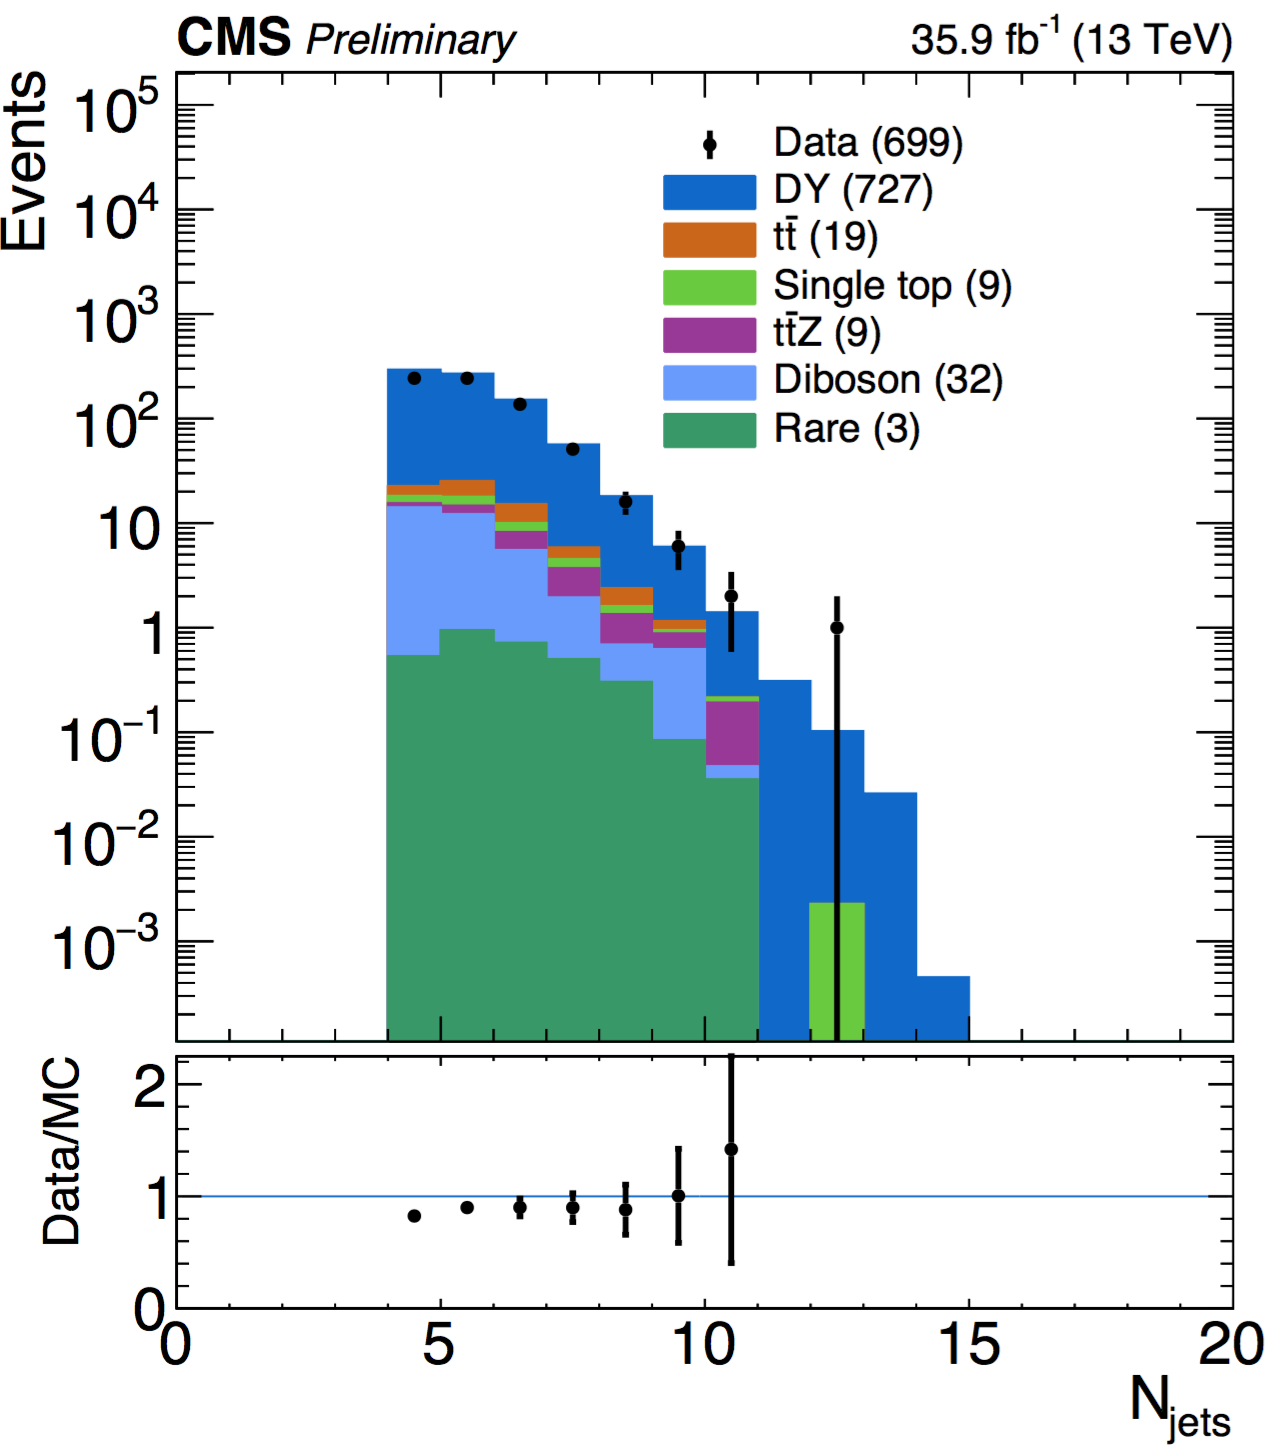
\includegraphics[width=0.4\textwidth]{NjetsShapeCorr.png}
\end{center}
\vspace{-1em}
\caption[$N_{jet}$ distribution in the tight $\mu\mu$ control region after $S_\gamma$ corrections.]{$N_{jet}$ distribution in the tight $\mu\mu$ control region after $S_\gamma$ corrections.}
\label{NjetsShapeCorr}
\end{figure}

The effect of the $S_{\gamma}$($N_j$) scale factor is shown for various distributions. These results show that the overall agreement between data and simulation improves after applying the corresponding shape corrections.

\begin{figure}[H]
\begin{center}
\begin{minipage}[b]{0.45\textwidth}
    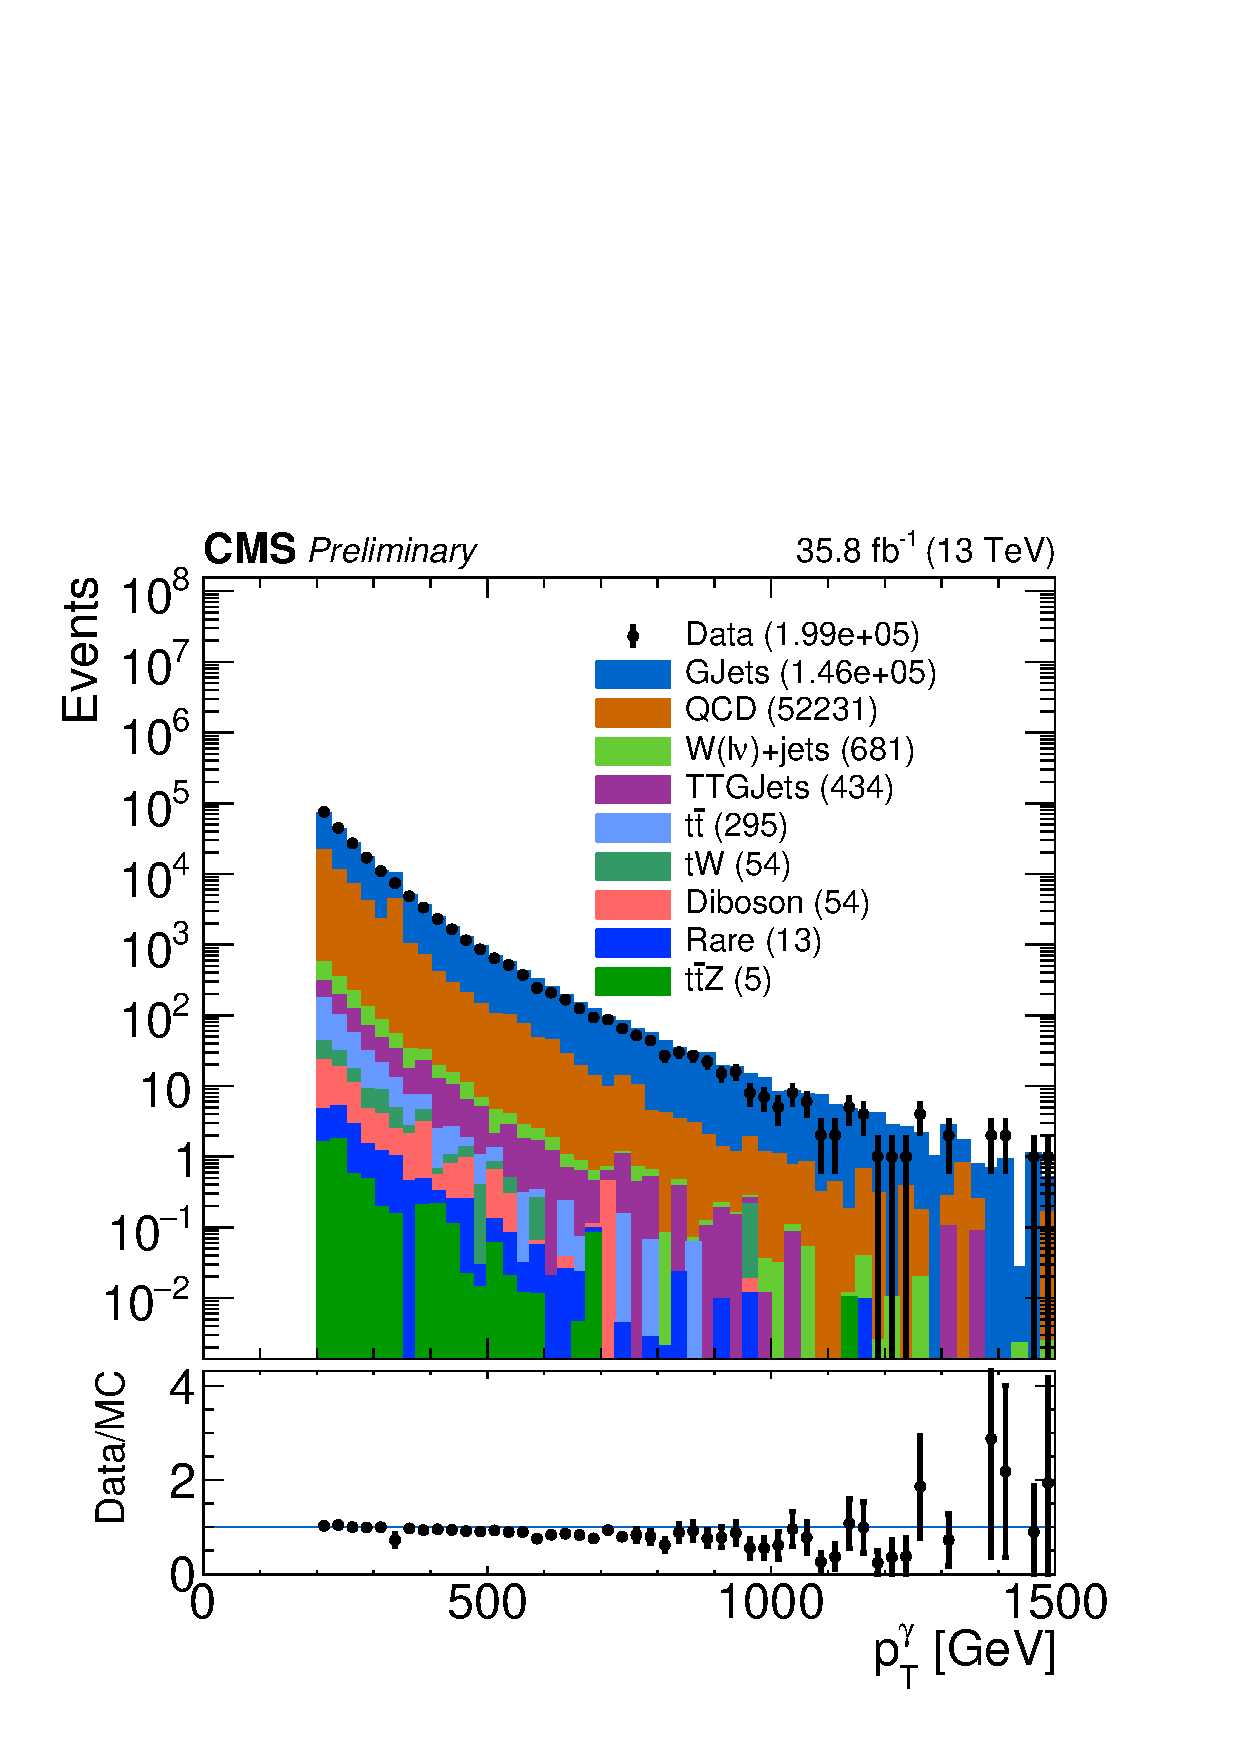
\includegraphics[width=\textwidth]{dataMC_PhotonPt_Wgt_LooseLepVeto.pdf}
\end{minipage}
\begin{minipage}[b]{0.45\textwidth}
    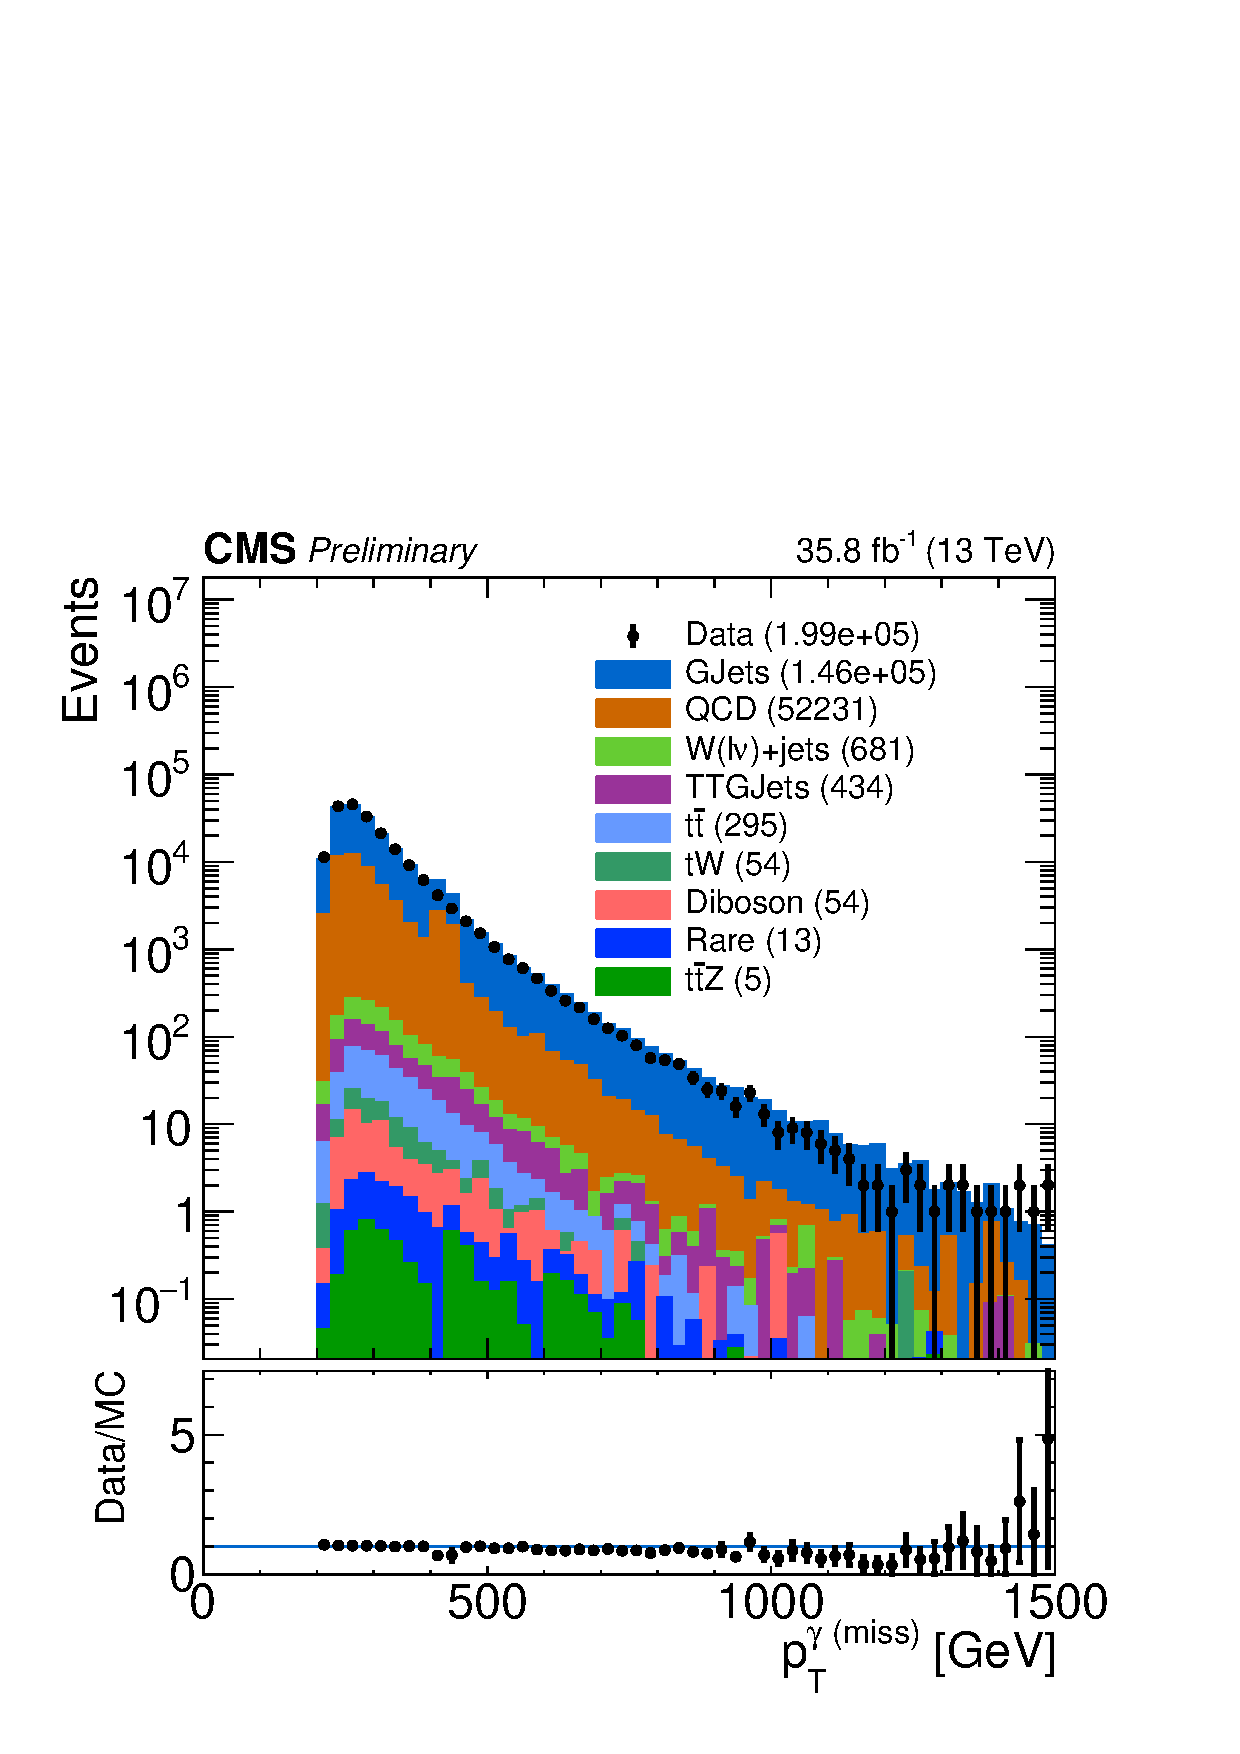
\includegraphics[width=\textwidth]{dataMC_MetGamma_Wgt_LooseLepVeto.pdf}
\end{minipage}
\end{center}
\vspace{-1em}
\caption{$p_\text{T}^\gamma$ (left) and $p_\text{T}^{\gamma (miss)}$ (right) distributions after applying the $S_\gamma$($N_j$) scale factor. Comparing to \autoref{PtMetPt}, an improvement in the agreement between data/MC can be observed.}
\label{PtMetPtCorr}
\end{figure}

\vspace {1em}

\begin{figure}[H]
\begin{center}
\begin{minipage}[b]{0.45\textwidth}
    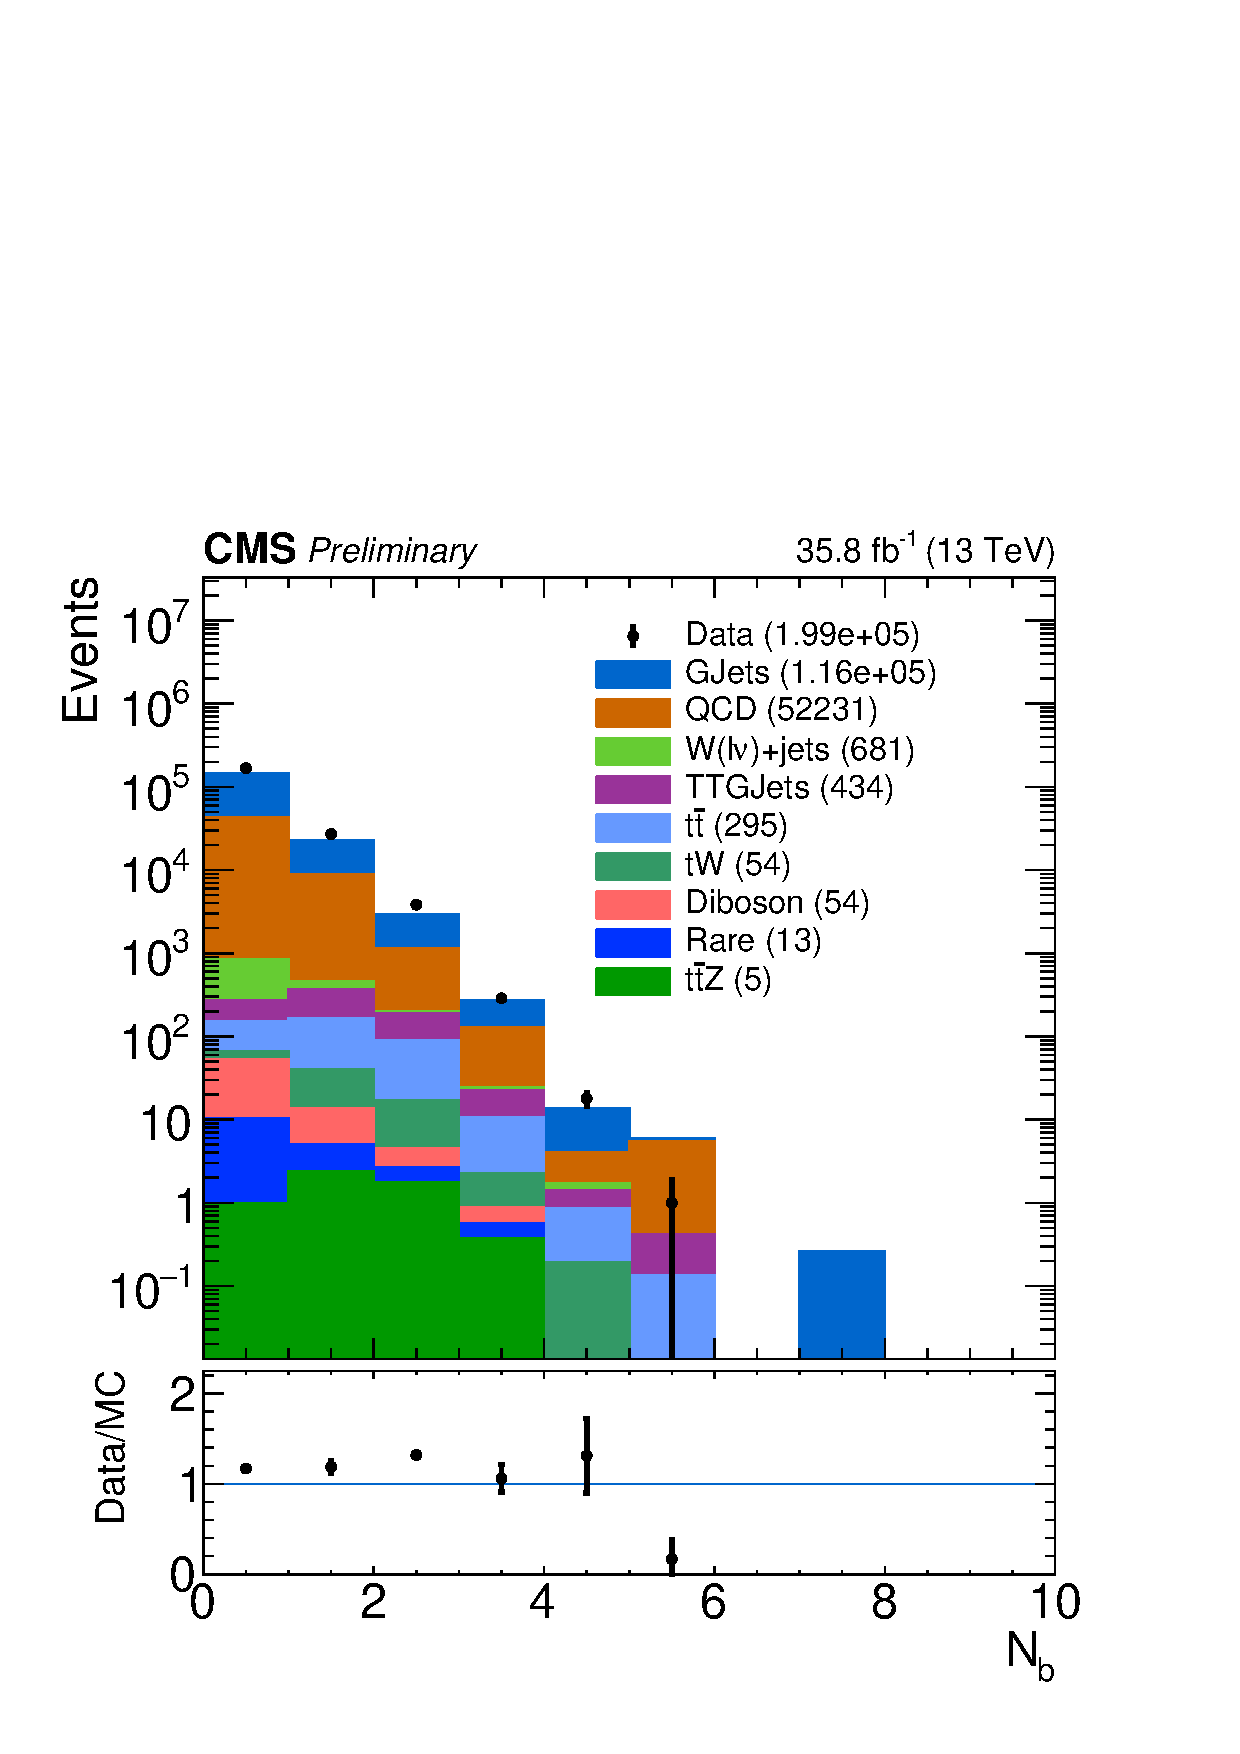
\includegraphics[width=\textwidth]{dataMC_Photon_nb_Log_LooseLepVeto.pdf}
\end{minipage}
\begin{minipage}[b]{0.45\textwidth}
    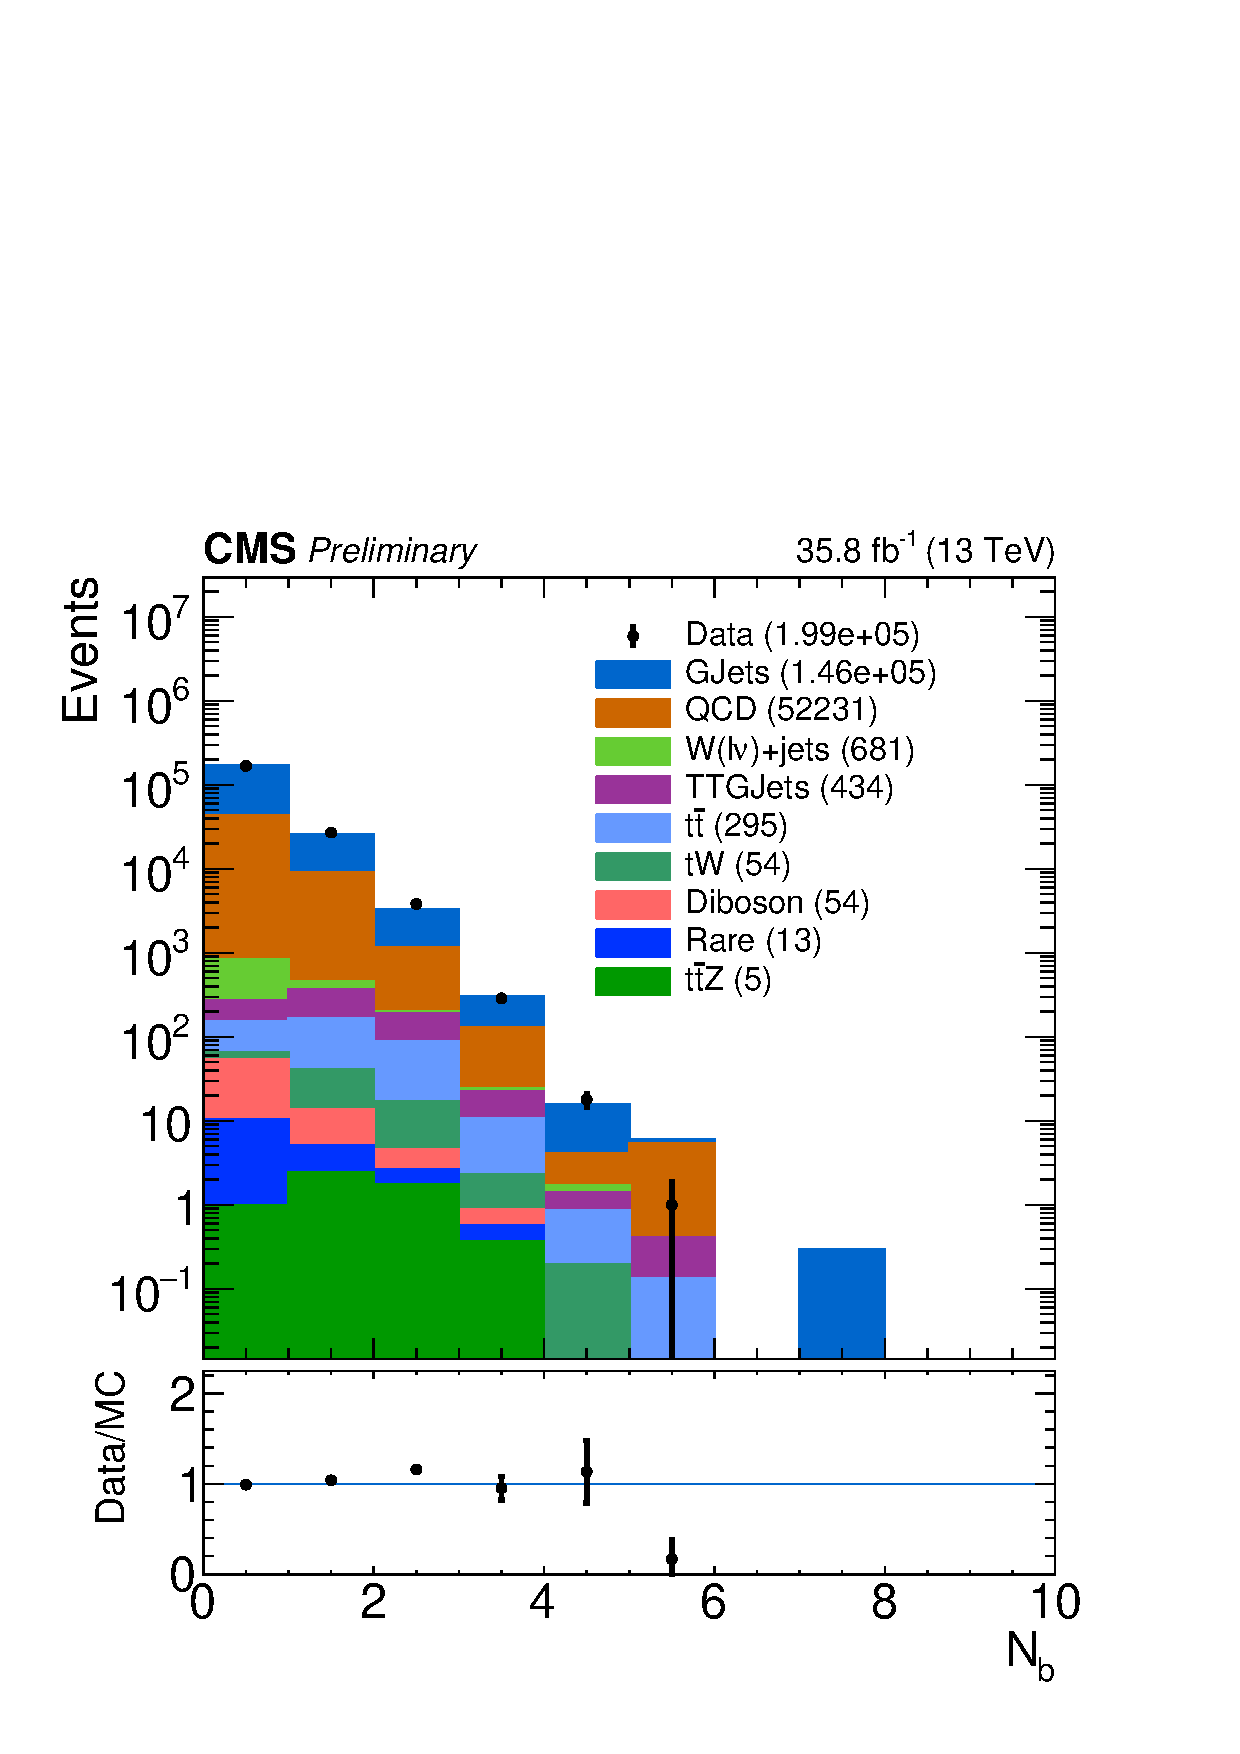
\includegraphics[width=\textwidth]{dataMC_Photon_nb_Log_Wgt_LooseLepVeto.pdf}
\end{minipage}
\end{center}
\vspace{-1em}
\caption{$N_b$ distribution before (left) and after (right) applying the $S_\gamma$($N_j$) scale factor. }
\end{figure}

%\vspace {1em}

\begin{figure}[tb]
\begin{center}
\begin{minipage}[b]{0.45\textwidth}
    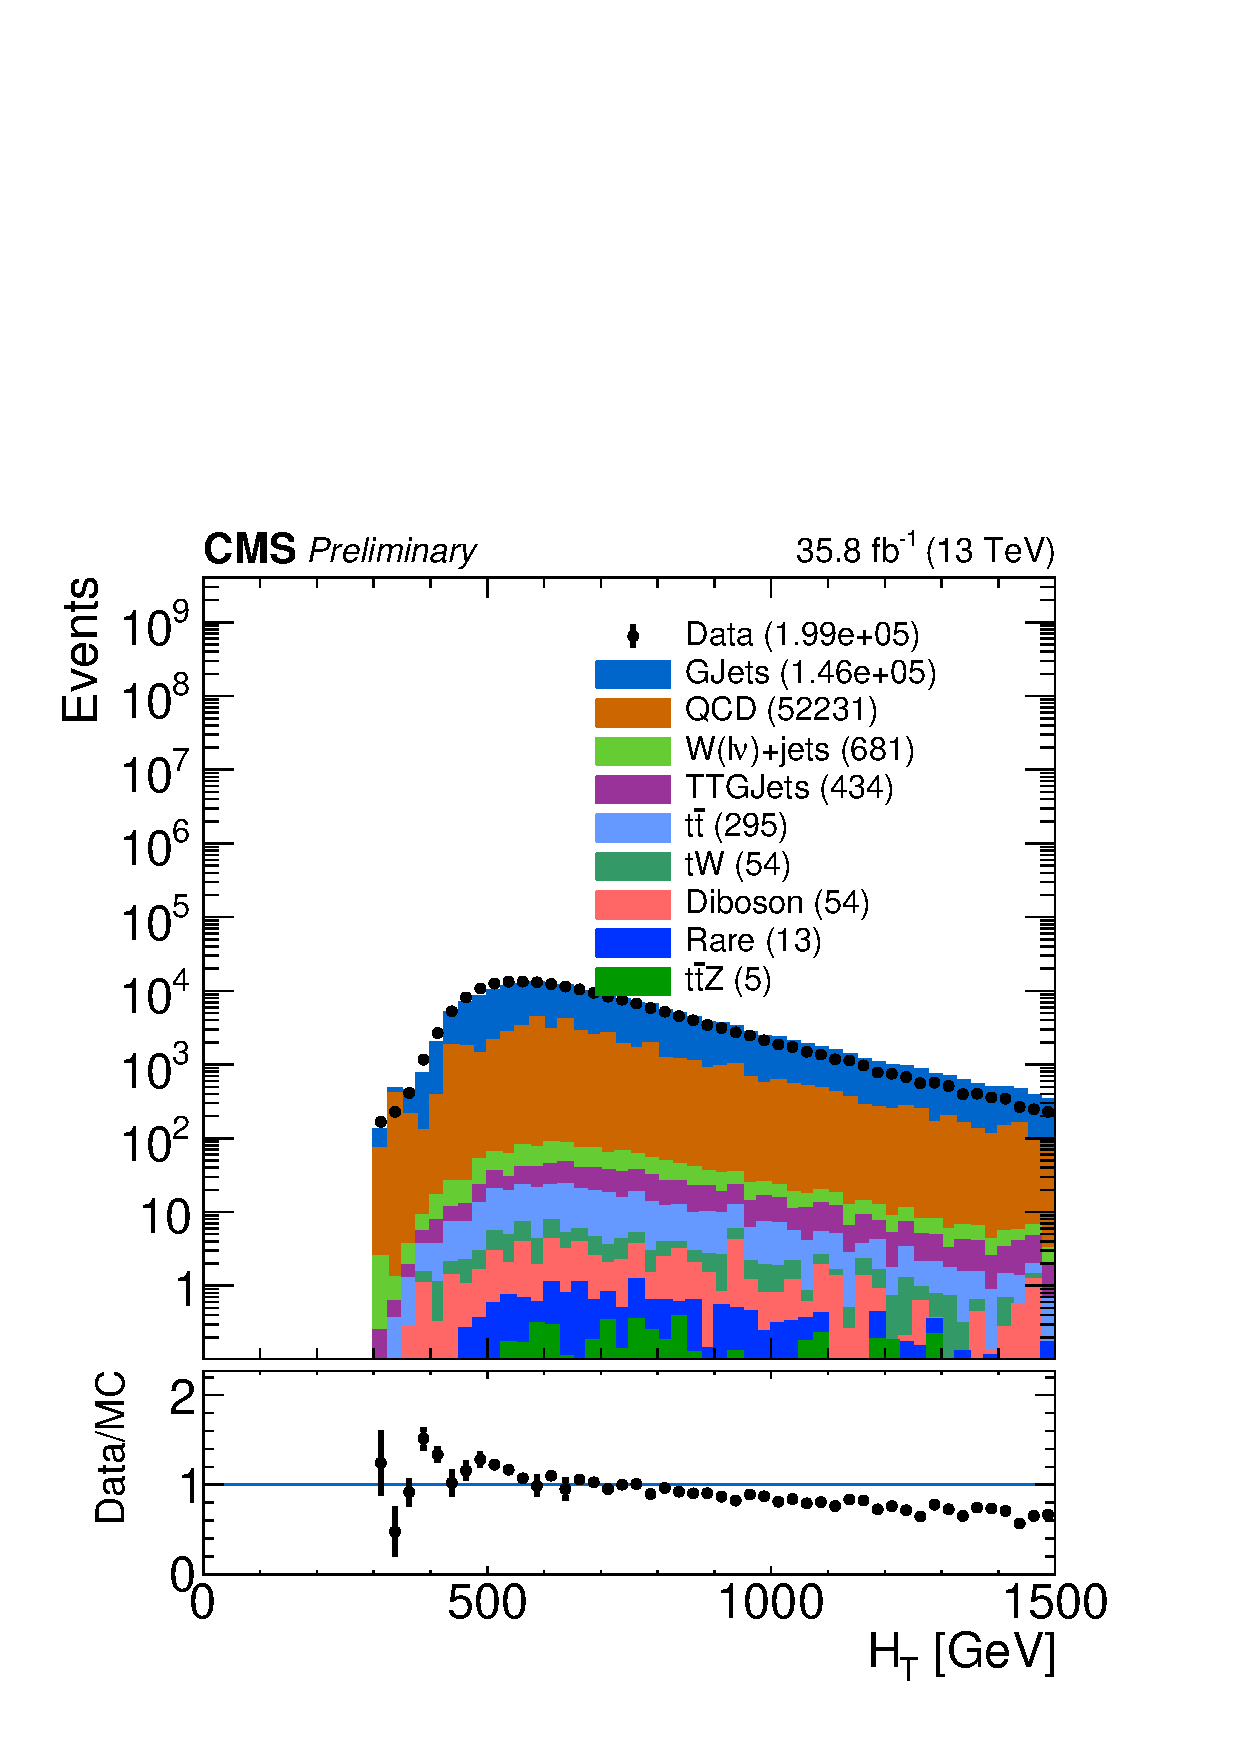
\includegraphics[width=\textwidth]{dataMC_Photon_ht_Wgt_LooseLepVeto.pdf}
\end{minipage}
\begin{minipage}[b]{0.45\textwidth}
    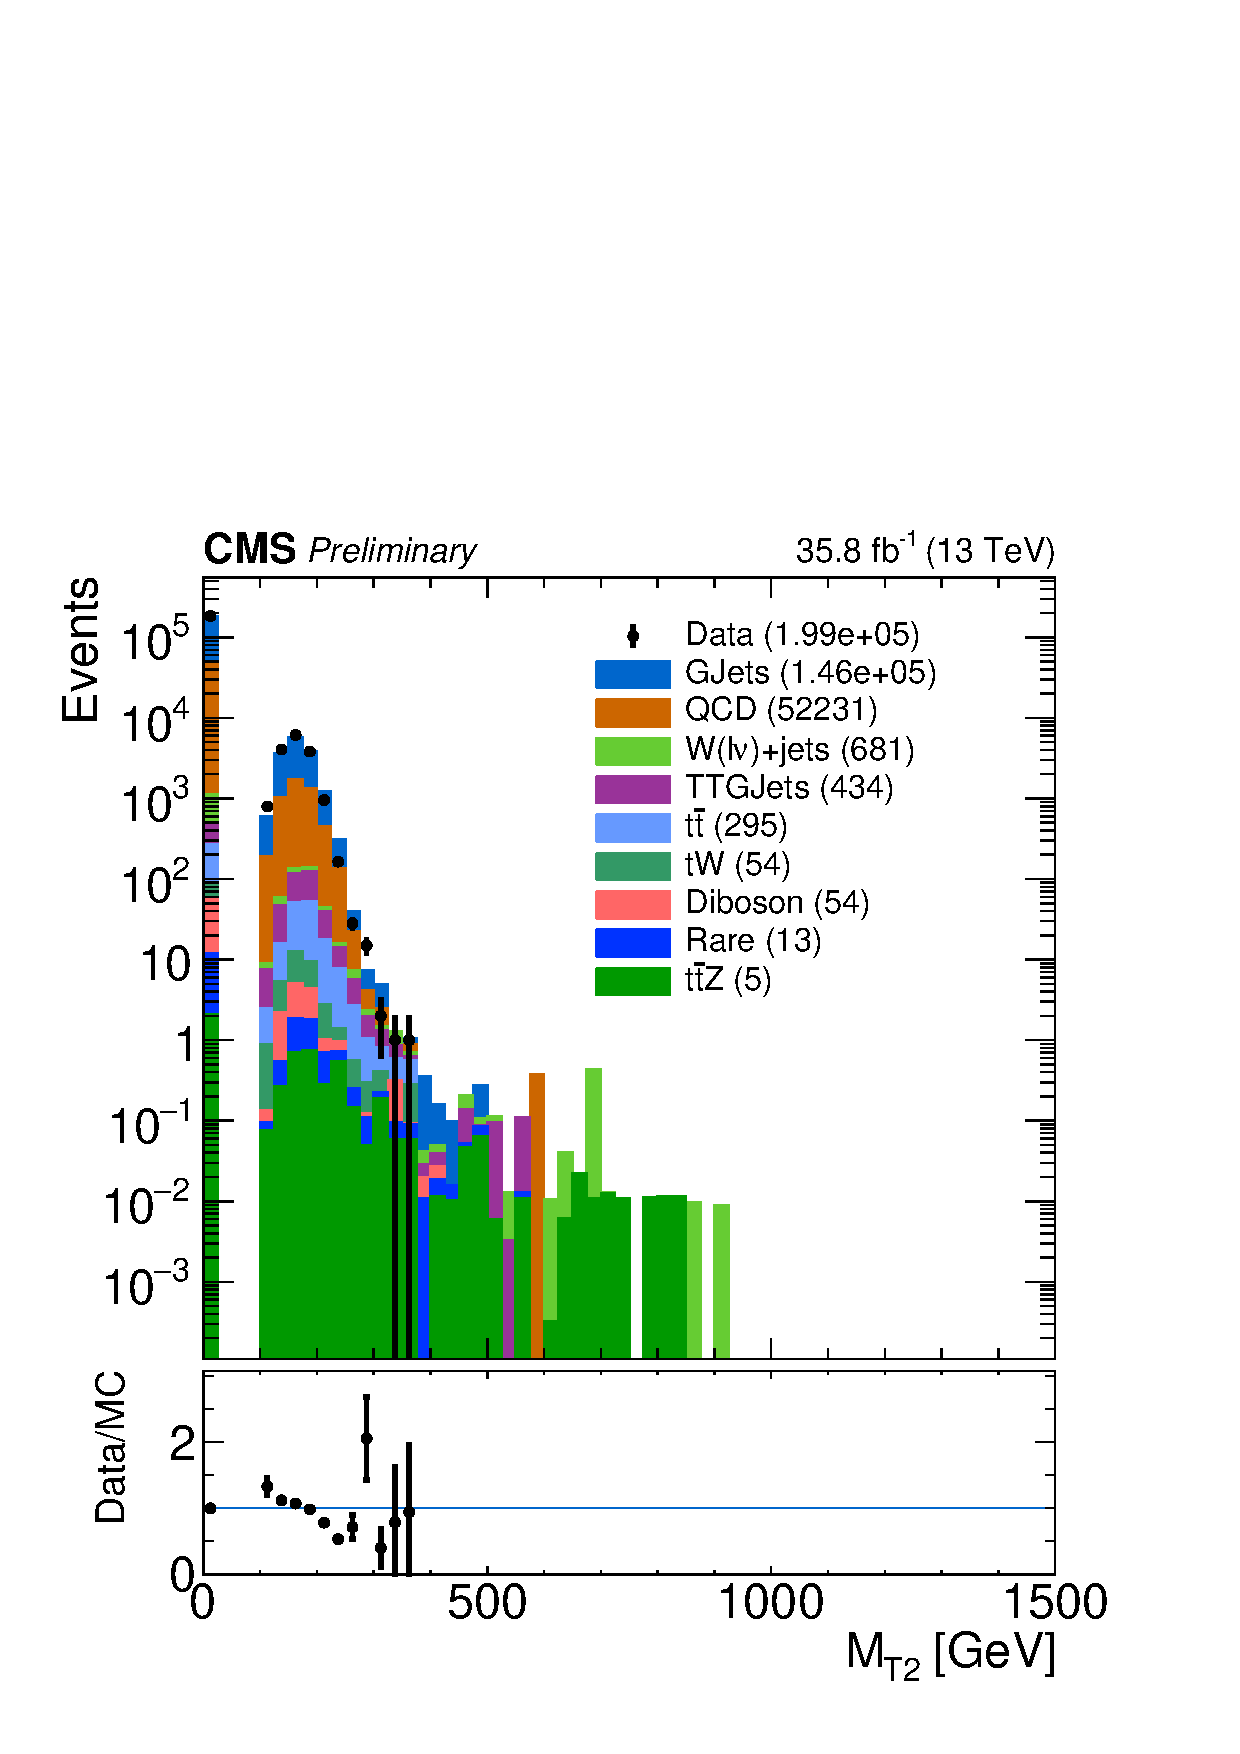
\includegraphics[width=\textwidth]{dataMC_Photon_mt2_Wgt_LooseLepVeto.pdf}
\end{minipage}
\end{center}
\vspace{-1em}
\caption{$H_\text{T}$ and $m_\text{T2}$ distributions applying the $S_\gamma$($N_j$) scale factor. }
\end{figure}

\subsection{Normalization Correction Using the tight Z$\rightarrow\mu^{+}\mu^{-}$ Control Sample}\label{tightmumu}

In order to constrain the normalization of the Z$\rightarrow\nu\bar{\nu}$ simulation sample, a normalization correction factor $R_{norm}$ is calculated from the tight $\mu\mu$ control region defined in \autoref{tightmumu}. Two categories are considered: the zero b-tagged jet category ($N_b = 0$), and the $\geq 1$ b-tagged jet category ($N_b \geq 1$). Both of these categories are statistically consistent with each other but the inclusive region ($N_b \geq 0$) has a lower overall uncertainty. The method used to calculate the normalization scale factor requires that the $N_j$-dependent shape correction factors already be applied. Then, the $R_{norm}$ factor can be extracted from the ratio of the total event yield in data to that in the simulation. This factor is found to be:

\begingroup
	\begin{center}
		$R_{norm} = 1.070 \pm 0.085$,
	\end{center}
\endgroup

\noindent where the uncertainty includes only the associated statistical uncertainties on data and simulation. This uncertainty is found to be propagated to the final background prediction, see \autoref{systematics}.\\

\begin{figure}[H]
\begin{center}
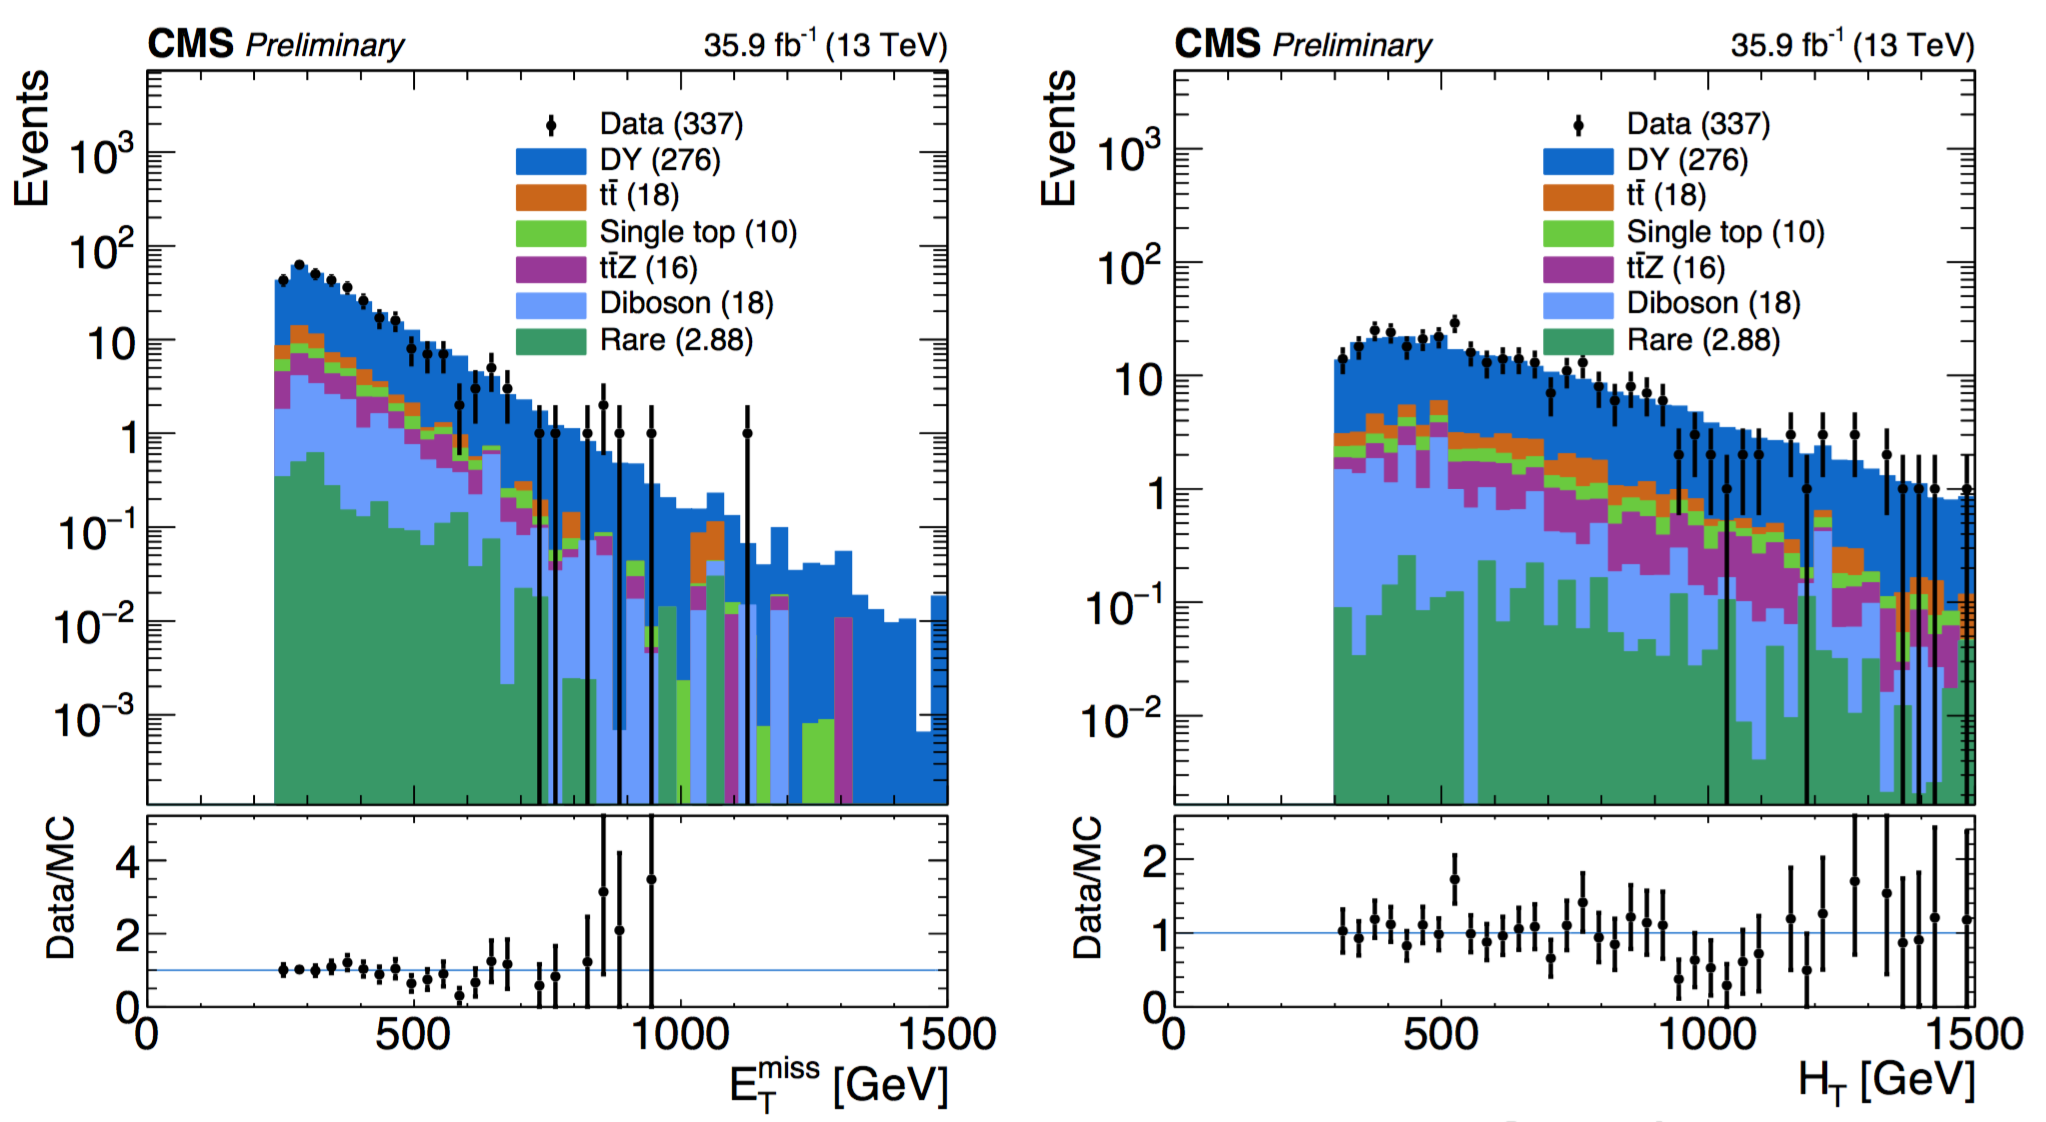
\includegraphics[width=\textwidth]{Rnorm1}
\end{center}
\vspace{-1em}
\caption{Shown are data/MC comparisons for the $p_\text{T}^{miss}$ (left) and $H_\text{T}$ (right) distributions after applying both the $N_j$-dependent shape corrections ($S_\gamma$) and the global normalization scale factor ($R_{norm}$).}
\label{Rnorm1}
\end{figure}

\vspace{1em}

Data/MC comparisons are shown in \autoref{Rnorm1} and \autoref{Rnorm2} after applying $R_{norm}$ for several distributions in the study. With this final global scale factor all the required ingredients for the central value of the Z$\rightarrow\nu\bar{\nu}$ background prediction are obtained. 

\begin{figure}[H]
\begin{center}
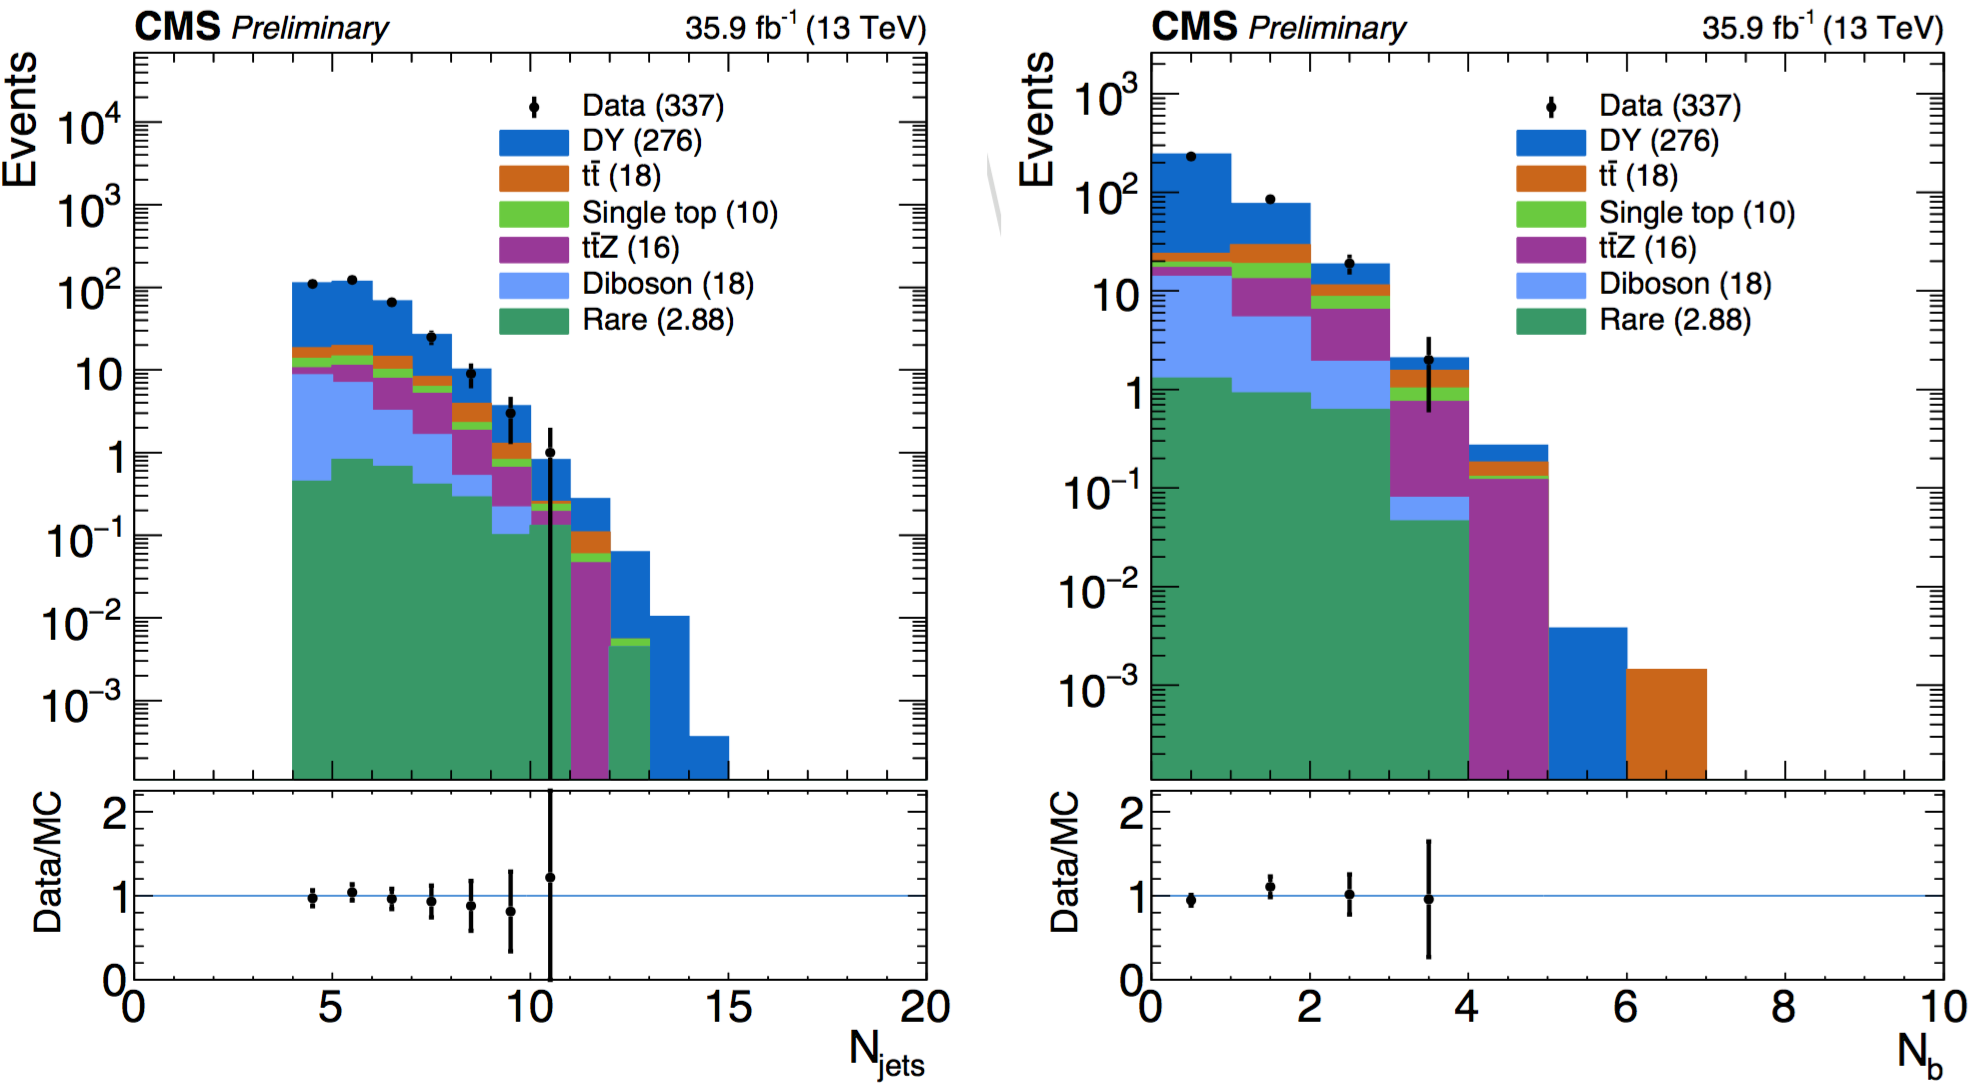
\includegraphics[width=\textwidth]{Rnorm2}
\end{center}
\vspace{-1em}
\caption{Shown are data/MC comparisons for the $N_j$ (left) and $N_b$ (right) distributions after applying both the $N_j$-dependent shape corrections ($S_\gamma$) and the global normalization scale factor ($R_{norm}$).}
\label{Rnorm2}
\end{figure}

\section{Results}

In this section the results for the final estimation of the of the Z$\rightarrow\nu\bar{\nu}$ are presented. The current study includes preliminary results using only data obtained at the CMS detector during 2016. The results for this study are intended to confirm the assumption that the additional $\gamma+$jets control region introduced in this analysis reduce the overall uncertainties obtained in the 2016 analyses (described in \autoref{AnalysisChap}). Furthermore, this study is intended as a benchmark for future analyses of the SUSY stop group based in Fermilab and will be the method used for the 2017 CMS data.

\subsection{Systematics}\label{systematics}

Two categories of uncertainties for the Z$\rightarrow\nu\bar{\nu}$ prediction are considered: uncertainties that are associated to the use of MC simulation and the uncertainties specifically associated to the background prediction method. Several sources are acknowledged in the first category mentioned such as PDF and renormalization/factorization scale choices, jet and $p_\text{T}^{miss}$ energy scale uncertainties b-tag scale factor uncertainties, and trigger efficiency uncertainties. Given that the simulation sample is normalized to data in the tight control region, uncertainties associated with the luminosity and cross-section are excluded. In addition, the overall Z$\rightarrow\nu\bar{\nu}$ statistical uncertainty from MC simulation is also taken into account.\\

\begin{figure}[H]
\begin{center}
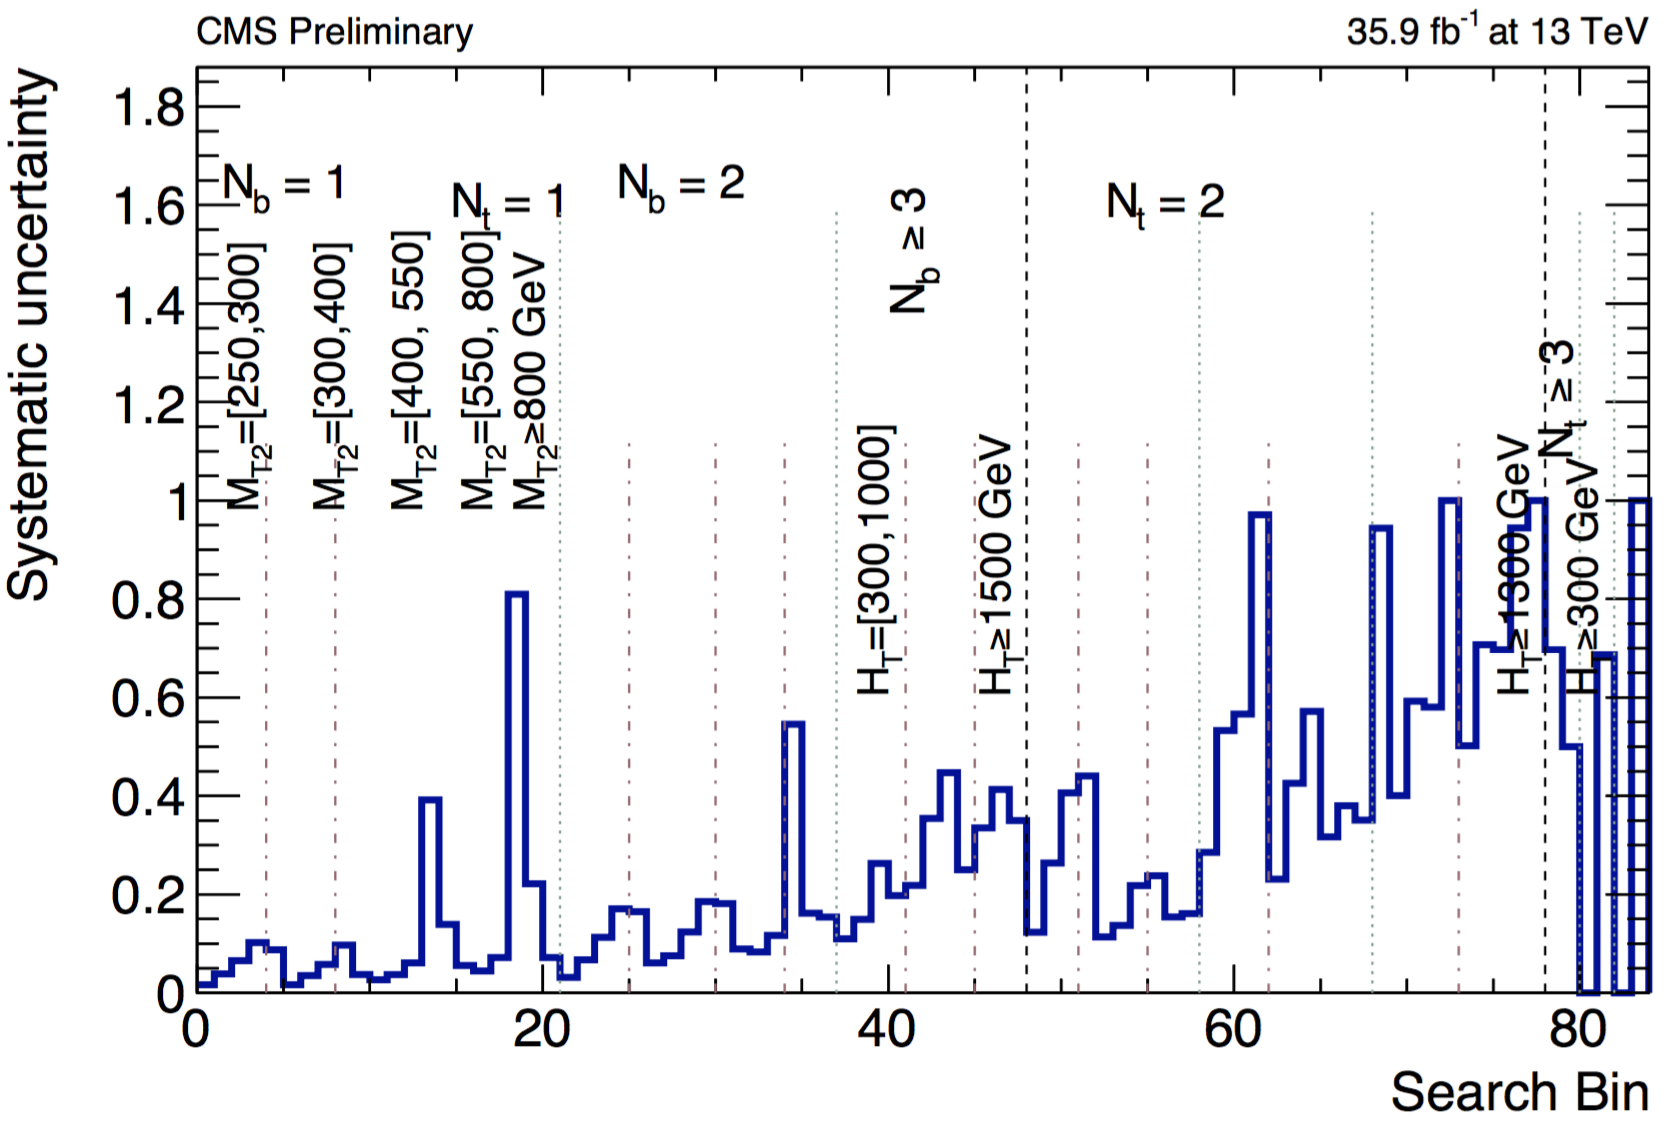
\includegraphics[width=0.8\textwidth]{UncZnunu}
\end{center}
\vspace{-1em}
\caption{Systematic uncertainty in the final prediction, as a function of the search bin, associated to the MC statistics.}
\label{UncZnunu}
\end{figure}

The statistical uncertainty associated with each bin in the MC is propagated as a systematic uncertainty. The relative uncertainty per bin can be see in \autoref{UncZnunu}. It shows that the uncertainties for the MC vary from as low as 1\% up to 81\% and even 100\% in some regions. Since the final estimation is scaled using the global normalization factor from the tight $\mu\mu$ control region ($R_{norm}$), the total uncertainty, due to limited amounts of events in data, is propagated in the final prediction. This is also true for the $S_\gamma$($N_j$) scale factor, in which the residual differences in search variables other than $N_j$ are evaluated in the loose photon control region. Both the uncertainty arising from the $N_j$ re-weighting as well as the residual differences are evaluated together. The uncertainty from $R_{norm}$ is propagated as a flat value of 7.9\% uncertainty per each search bin.

\subsection{Z$\rightarrow\nu\bar{\nu}$ Estimation for the Search Bins}

The final estimation for the Z$\rightarrow\nu\bar{\nu}$ background calculated for all 84 search bins is shown in \autoref{results}. The statistical uncertainty in bins that have zero events is treated as the average weight (the sum of the weights squared over the weight) times the poisson error on 0 which is 1.8. This average weight is calculated on the basis of a relaxed cut in which $N_b \geq 2$ is required. For comparison, a cut in which $N_t > 2$ where two tops are fake for the Z$\rightarrow\nu\bar{\nu}$ is used.

\begin{figure}[H]
\begin{center}
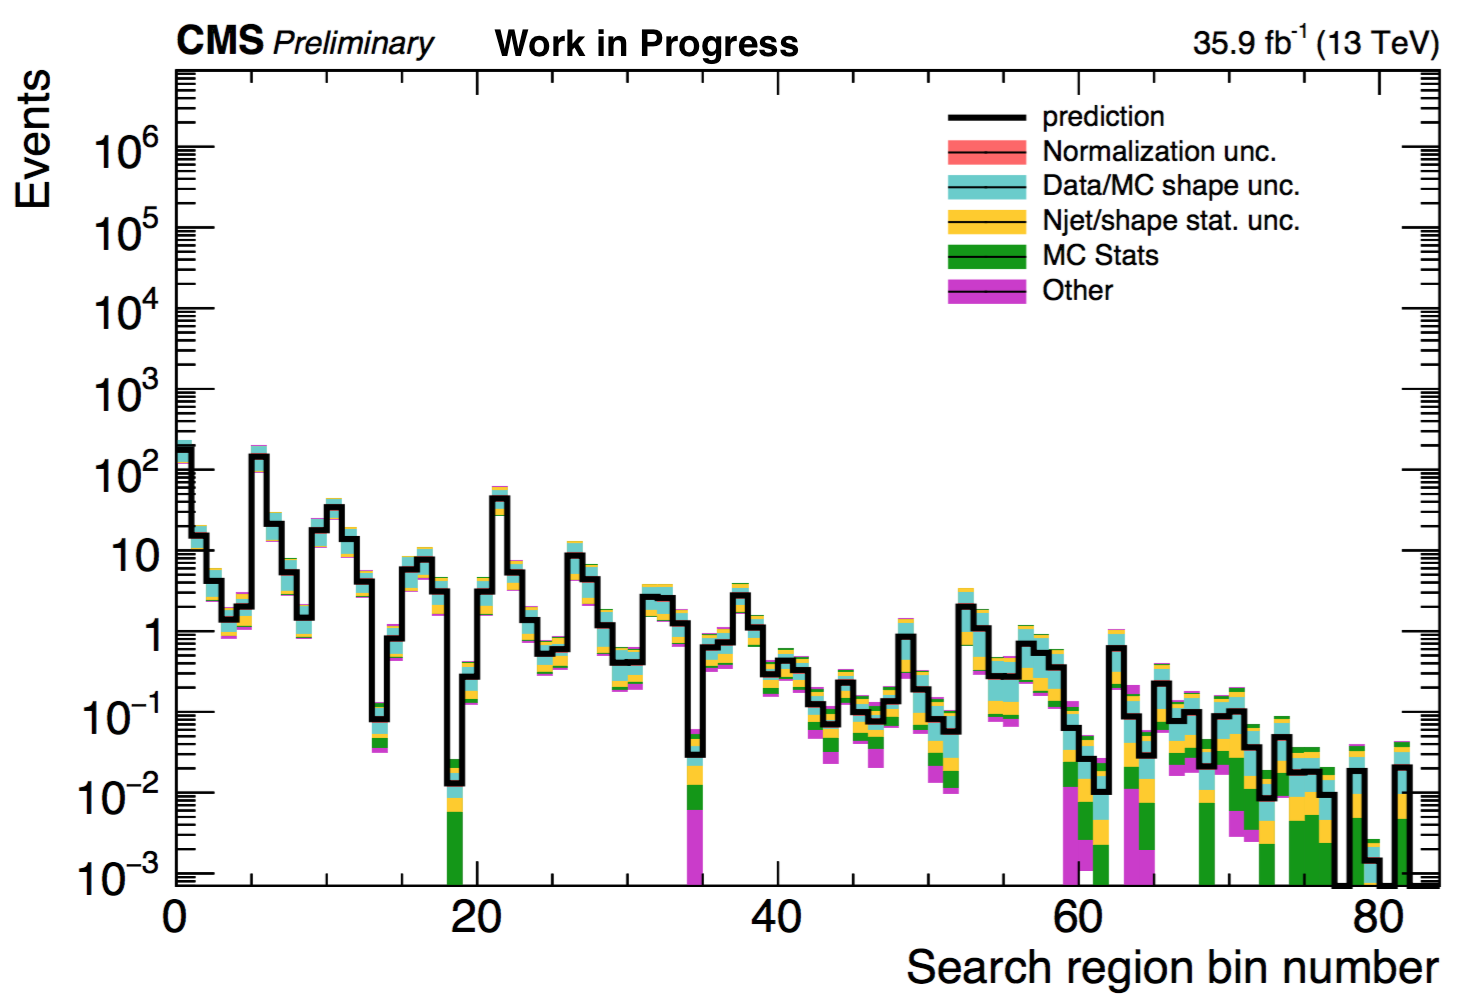
\includegraphics[width=0.8\textwidth]{Results.png}
\end{center}
\vspace{-1em}
\caption{Z$\rightarrow\nu\bar{\nu}$ background prediction for all search bins, including the breakdown of the various uncertainties.}
\label{results}
\end{figure}

